\documentclass[letterpaper, italian]{report}
\usepackage[utf8]{inputenc}
\usepackage{csvsimple}
\usepackage[hidelinks, unicode]{hyperref}
\usepackage{graphicx}
\usepackage[T1]{fontenc}
\usepackage{contour}
\usepackage{ulem}
\usepackage{bookmark}
\usepackage{enumitem}
\usepackage{longtable}
\usepackage{booktabs}
\usepackage{float}
\usepackage{xcolor}
\usepackage{typearea}
\usepackage[letterpaper]{geometry}
\usepackage{lipsum}
\usepackage{makecell}
\usepackage{caption}

\makeatletter % removes Chpater N from Chapter title without using titlesec, can be very useful in KOMA environments
\def\@makechapterhead#1{%
  \vspace*{0\p@}%
  {\parindent \z@ \centering \normalfont
    % \ifnum \c@secnumdepth >\m@ne
    %     \huge\bfseries
    %     % \@chapapp\space % removed
    %     \thechapter
    %     \nobreakspace{}% \par\nobreak\vskip 20\p@ % replaced
    % \fi
    % \interlinepenalty\@M
    \huge % \Huge % replaced
    \bfseries #1\par\nobreak
    \vskip 40\p@
  }}
\makeatother

\renewcommand{\ULdepth}{1.8pt} % underline depth
\contourlength{0.8pt}

\newcommand{\myuline}[1]{% better underline
  \uline{\phantom{#1}}%
  \llap{\contour{white}{#1}}%
}

\newcommand{\uselandscape}{% to insert landscape pages inside portrait document
  \cleardoublepage
  \KOMAoptions{paper=landscape}%
  \recalctypearea
  \areaset{2.0\textwidth}{2.0\textheight}% adjust here: \areaset{<text body width>}{<text body height>}
}

\AtBeginDocument{%
  \storeareas\normalpapersize
}
\BeforeRestoreareas{\cleardoublepage}

\renewcommand{\thesection}{\arabic{section}} % removes reference of \chapter to avoid "0."
\renewcommand{\thesubsection}{\thesection.\alph{subsection}.1}
% \titleformat{\chapter}{\normalfont\huge}{\thechapter}{20pt}{\huge\it}

\title{
    \leavevmode{
\includegraphics[width=0.8\textwidth]{../resources/img/Universita-degli-studi-di-torino-logo.png}\newline\newline}\\
    Cat \& Ring \\
    \large Gestire i Compiti della Cucina
}
\author{Eduard Antonovic Occhipinti, Riccardo Cardona}

\begin{document}

\maketitle

\tableofcontents

\part{Requisiti}
\chapter{UC Dettagliato}

\section*{Informazioni generali}
\textbf{Nome caso d'uso}{: Gestire le ricette}\newline
\textbf{Portata}{: Sistema}\newline
\textbf{Livello}{: Obiettivo utente}\newline
\textbf{Attore primario}{: Cuoco}\newline
\textbf{Parti Interessate}\newline
\textbf{Pre-condizioni}{: L'attore deve essere autenticato come Cuoco}\newline
\textbf{Garanzie di successo o post-condizioni}{: La procedura di cucina è salvata}

\small
\section*{Scenario Principale di Successo}\addcontentsline{toc}{section}{Scenario Principale di Successo}
\def\arraystretch{1.55}%  1 is the default, change whatever you need
\begin{tabular}{|c|p{7cm}|p{6.5cm}|}
      \hline\bfseries \# & \bfseries Attore                                                                                                                 & \bfseries Sistema                                         \\\hline

      1                  & Crea una nuova procedura di cucina passandogli un nome specificando se la procedura è una ricetta o una preparazione             & Registra la nuova procedura e la salva nel ricettario     \\\hline
      2                  & Opzionalmente aggiunge uno o più passi alla procedura e opzionalmente specificando le ripetizioni e se è preparabile in anticipo & Registra i passi della procedura                          \\\hline
      \multicolumn{3}{|r|}{\textit{Se desidera creare una variante di una ricetta torna al passo 1}}                                                                                                                    \\\hline
      3                  & Annota gli ingredienti con opzionalmente le dosi                                                                                 &                                                           \\\hline
      \multicolumn{3}{|r|}{\textit{Ripete finché non è soddisfatto}}                                                                                                                                                    \\\hline
      4                  & Opzionalmente consulta il ricettario                                                                                             & Fornisce il ricettario                                    \\\hline
      \multicolumn{3}{|r|}{\textit{Se desidera creare una variante di una preparazione torna al passo 1}}                                                                                                               \\\hline
      5                  & Opzionalmente usa una preparazione del ricettario come ingrediente della procedura                                               & Registra la preparazione come ingrediente della procedura \\\hline
      6                  & Opzionalmente modifica un passo della procedura,Registra il nuovo passo della procedura                                          &                                                           \\\hline
      7                  & Opzionalmente dettaglia la procedura inserendo le porzioni, la tempistica e annota se può essere preparata in anticipo           & Registra le nuove informazioni alla procedura             \\\hline
      \multicolumn{3}{|r|}{\textit{Se desidera torna al passo 2 altrimenti prosegue}}                                                                                                                                   \\\hline
      8                  & Pubblica la procedura nel ricettario opzionalmente modificando il titolo                                                         & La procedura diventa visibile a tutti nel ricettario      \\\hline
\end{tabular}

\addcontentsline{toc}{subsection}{Estensioni 1}
\begin{table}[H]\caption*{Estensione 1a}
      \small
      \begin{tabular}{|c|p{7cm}|p{6.23cm}|}
            \hline\bfseries \# & \bfseries Attore                                                                & \bfseries Sistema           \\\hline
            1a.1               & Crea una variante di una procedura dandogli un nome riferito a quello originale & Registra la nuova procedura \\\hline
      \end{tabular}
\end{table}

\begin{table}[H]\caption*{Estensione 1b}
      \small
      \begin{tabular}{|c|p{7cm}|p{6.23cm}|}
            \hline\bfseries \# & \bfseries Attore                   & \bfseries Sistema                                                                             \\\hline
            1b.1               & Apri una procedura per modificarla & Fornisce la procedura richiesta rendendola non più visibile a tutti e utilizzabile in un menù \\\hline
      \end{tabular}
\end{table}

\begin{table}[H]\caption*{Estensione 1c}
      \small
      \begin{tabular}{|c|p{7cm}|p{6.24cm}|}
            \hline\bfseries \# & \bfseries Attore                & \bfseries Sistema                    \\\hline
            1c.1               & Elimina una procedura esistente & Elimina una procedura dal ricettario \\\hline
      \end{tabular}
\end{table}

\addcontentsline{toc}{subsection}{\indent\color{red}{Eccezioni 1}}
\begin{table}[H]\centering\color{red}\caption*{Eccezione 1b.1a}
      \small
      \begin{tabular}{|c|p{7cm}|p{5.8cm}|}
            \hline\bfseries \# & \bfseries Attore                   & \bfseries Sistema                                  \\\hline
            1b.1a.1            & Apri una procedura per modificarla & La procedura serve per un menù in uno in un evento \\\hline
            \multicolumn{3}{|r|}{\textit{Termina il caso d'uso}}                                                         \\\hline
      \end{tabular}
\end{table}

\begin{table}[H]\centering\color{red}\caption*{Eccezione 1b.1b}
      \small
      \begin{tabular}{|c|p{7cm}|p{5.8cm}|}
            \hline\bfseries \# & \bfseries Attore                   & \bfseries Sistema                                                                                          \\\hline
            1b.1b.1            & Apri una procedura per modificarla & La procedura non è di proprietà dell’attore che sta cercando di modificarlo pertanto non si può proseguire \\\hline
            \multicolumn{3}{|r|}{\textit{Termina il caso d'uso}}                                                                                                                 \\\hline
      \end{tabular}
\end{table}

\begin{table}[H]\centering\color{red}\caption*{Eccezione 1c.1a}
      \small
      \begin{tabular}{|c|p{7cm}|p{5.8cm}|}
            \hline\bfseries \# & \bfseries Attore                & \bfseries Sistema                                  \\\hline
            1c.1a.1            & Elimina una procedura esistente & La procedura serve per un menù in uno in un evento \\\hline
            \multicolumn{3}{|r|}{\textit{Termina il caso d'uso}}                                                      \\\hline
      \end{tabular}
\end{table}

\begin{table}[H]\centering\color{red}\caption*{Eccezione 1c.1b}
      \small
      \begin{tabular}{|c|p{7cm}|p{5.8cm}|}
            \hline\bfseries \# & \bfseries Attore                & \bfseries Sistema                                                                                         \\\hline
            1c.1b.1            & Elimina una procedura esistente & La procedura non è di proprietà dell’attore che sta cercando di eliminarlo pertanto non si può proseguire \\\hline
            \multicolumn{3}{|r|}{\textit{Termina il caso d'uso}}                                                                                                             \\\hline
      \end{tabular}
\end{table}

\addcontentsline{toc}{subsection}{Estensioni 2}
\begin{table}[H]\centering\caption*{Estensione 2a}
      \small
      \begin{tabular}{|c|p{7cm}|p{6.24cm}|}
            \hline\bfseries \# & \bfseries Attore                                                                                                                                                                   & \bfseries Sistema                                         \\\hline
            2a.1               & Opzionalmente crea un raggruppamento di passi dati uno o più passi semplici da inserire nella procedure e opzionalmente specificando le ripetizioni e se è preparabile in anticipo & Registra il nuovo raggruppamento di passi nella procedura \\\hline
            \multicolumn{3}{|r|}{\textit{Se desidera creare una variante di una ricetta torna al passo 1}}                                                                                                                                                                      \\\hline
      \end{tabular}
\end{table}

\begin{table}[H]\centering\caption*{Estensione 2b}
      \small
      \begin{tabular}{|c|p{7cm}|p{6.24cm}|}
            \hline\bfseries \# & \bfseries Attore                                                                                                                                 & \bfseries Sistema                                          \\\hline
            2b.1               & Opzionalmente crea una variante di un passo inserendo 2 passi da inserire nella procedura e opzionalmente indicando se è preparabile in anticipo & Registra il nuovo raggruppamento di passi per la procedura \\\hline
            \multicolumn{3}{|r|}{\textit{Se desidera creare una variante di una ricetta torna al passo 1}}                                                                                                                                     \\\hline
      \end{tabular}
\end{table}

\addcontentsline{toc}{subsection}{Estensioni 3}
\begin{table}[H]\centering\caption*{Estensione 3a}
      \small
      \begin{tabular}{|c|p{7cm}|p{6.24cm}|}
            \hline\bfseries \# & \bfseries Attore                                   & \bfseries Sistema                                             \\\hline
            3a.1               & Modifico le dosi di un ingrediente della procedura & Registro la procedura con le dosi dell’ingrediente modificato \\\hline
      \end{tabular}
\end{table}

\begin{table}[H]\centering\caption*{Estensione 3b}
      \small
      \begin{tabular}{|c|p{7cm}|p{6.24cm}|}
            \hline\bfseries \# & \bfseries Attore                       & \bfseries Sistema                     \\\hline
            3b.1               & Elimino un ingrediente della procedura & Elimino l’ingrediente dalla procedura \\\hline
      \end{tabular}
\end{table}

\addcontentsline{toc}{subsection}{Estensioni 5}
\begin{table}[H]\centering\caption*{Estensione 5a}
      \small
      \begin{tabular}{|c|p{7cm}|p{6.24cm}|}
            \hline\bfseries \# & \bfseries Attore                       & \bfseries Sistema                                            \\\hline
            5a.1               & Elimino una procedura come ingrediente & Elimino la procedura come ingrediente della procedura creata \\\hline
      \end{tabular}
\end{table}

\addcontentsline{toc}{subsection}{Estensioni 6}
\begin{table}[H]\centering\caption*{Estensione 6a}
      \small
      \begin{tabular}{|c|p{7cm}|p{6.24cm}|}
            \hline\bfseries \# & \bfseries Attore                                          & \bfseries Sistema                                  \\\hline
            6a.1               & Opzionalmente modifico l’ordine dei passi della procedura & Registra il nuovo ordine dei passi nella procedura \\\hline
      \end{tabular}
\end{table}

\begin{table}[H]\centering\caption*{Estensione 6b}
      \small
      \begin{tabular}{|c|p{7cm}|p{6.24cm}|}
            \hline\bfseries \# & \bfseries Attore                               & \bfseries Sistema                \\\hline
            6b.1               & Opzionalmente elimino un passo della procedura & Elimino il passo della procedura \\\hline
      \end{tabular}
\end{table}

\addcontentsline{toc}{subsection}{Estensioni 7}
\begin{table}[H]\centering\caption*{Estensione 7a}
      \small
      \begin{tabular}{|c|p{7cm}|p{6.24cm}|}
            \hline\bfseries \# & \bfseries Attore                                  & \bfseries Sistema                               \\\hline
            7a.1               & Opzionalmente modifica i dettagli della procedura & Registra la procedura con i dettagli modificati \\\hline
      \end{tabular}
\end{table}

\begin{table}[H]\centering\caption*{Estensione 7b}
      \small
      \begin{tabular}{|c|p{7cm}|p{6.24cm}|}
            \hline\bfseries \# & \bfseries Attore                                      & \bfseries Sistema                     \\\hline
            7b.1               & Opzionalmente elimina una annotazione dalla procedura & Elimina l’annotazione dalla procedura \\\hline
      \end{tabular}
\end{table}

\begin{table}[H]\centering\caption*{Estensione 7c}
      \small
      \begin{tabular}{|c|p{7cm}|p{6.24cm}|}
            \hline\bfseries \# & \bfseries Attore                                                                                          & \bfseries Sistema                                     \\\hline
            7c.1               & Opzionalmente crea una procedura passando un nome e specificando se è una ricetta o una preparazione      & Registra la nuova procedura e la salva nel ricettario \\\hline
            7c.2               & Opzionalmente seleziono uno o più passi da inserire nella procedura appena creata                         & Registra i passi della procedura                      \\\hline
            7c.3               & Opzionalmente seleziono uno o più ingredienti con relative dosi da inserire nella procedura appena creata & Registra gli ingredienti della procedura              \\\hline
      \end{tabular}
\end{table}

\addcontentsline{toc}{subsection}{Estensioni 8}
\begin{table}[H]\centering\caption*{Estensione 8a}
      \small
      \begin{tabular}{|c|p{7cm}|p{6.24cm}|}
            \hline\bfseries \# & \bfseries Attore                                 & \bfseries Sistema \\\hline
            8a.1               & Conclude il lavoro senza pubblicare la procedura &                   \\\hline
      \end{tabular}
\end{table}
\normalsize

\uselandscape
\chapter{Modello di Dominio}
\begin{figure}[H]
      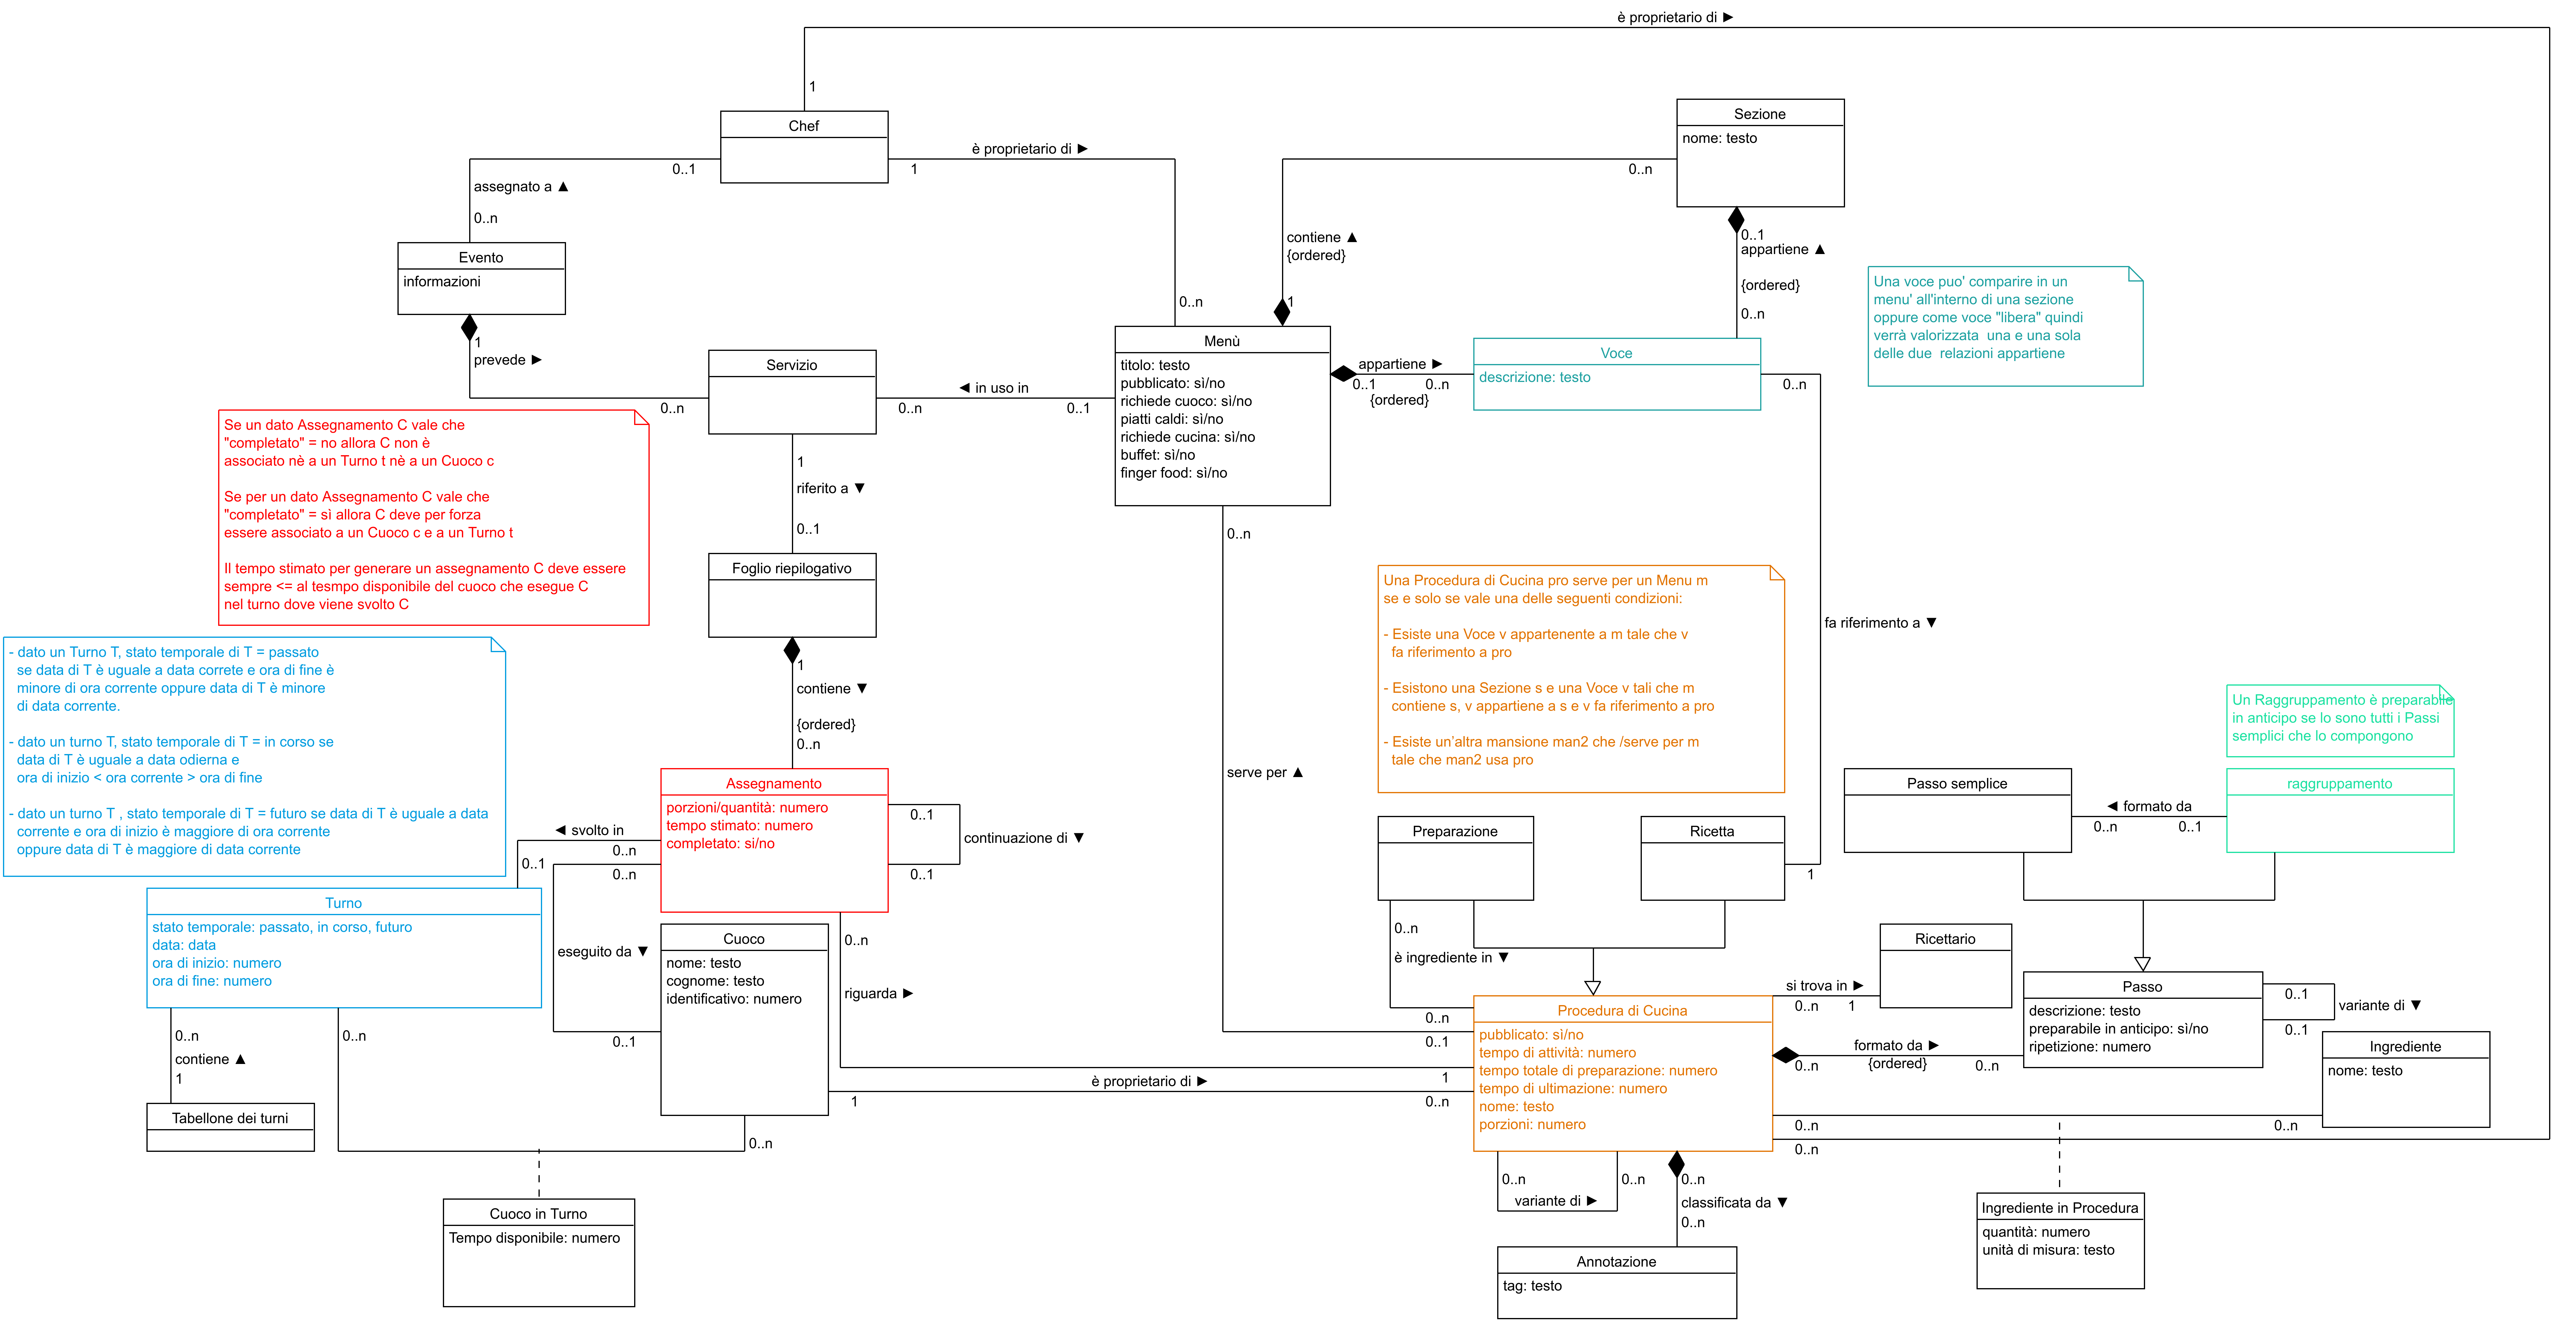
\includegraphics[width=\textwidth]{../resources/img/Domain Model.png}
\end{figure}
\normalpapersize

\clearpage
\chapter{Diagrammi di Sequenza di Sistema}
\section*{Scenario Principale di Successo}\addcontentsline{toc}{section}{Scenario Principale di Successo}
% includegraphics[width=\textwidth]{../resources/img/GCC/SSD.pdf}
\section*{Estensioni 1}\addcontentsline{toc}{subsection}{Estensioni 1}
% includegraphics[width=\textwidth]{../resources/img/GCC/SSD-ext1.pdf}
\section*{Estensioni 2}\addcontentsline{toc}{subsection}{Estensioni 2}
% includegraphics[width=\textwidth]{../resources/img/GCC/SSD-ex2.pdf}
\section*{Estensioni 5}\addcontentsline{toc}{subsection}{Estensioni 5}
% includegraphics[width=\textwidth]{../resources/img/GCC/SSD-ex5.pdf}



\chapter{Contratti delle Operazioni}
\textbf{Pre-condizione generale}{: l'utente è identificato come Cuoco o come Chef }\textit{c}

\section[creaProcedura]{\texorpdfstring{creaProcedura(\myuline{nome}: Testo, \myuline{èRicetta}: sì/no)}}\label{h.n5k8dzisnnko}
\textbf{Pre-condizioni:} -\newline
\textbf{Post-condizioni:}
\begin{itemize}[label=$-$, noitemsep]
	\item {[\textbf{Se} \myuline{èRicetta} == sì]}
	\setlist{nolistsep}
	\begin{itemize}[label=$-$, noitemsep]
		\item È stata creata un'istanza \textit{p} di Ricetta
		\item \textit{p.pubblicato} = no
		\item \textit{p.nome } = \myuline{nome}
	\end{itemize}
	\item {[\textbf{Se} \myuline{èRicetta} == no]}
	\setlist{nolistsep}
	\begin{itemize}[label=$-$, noitemsep]
		\item È stata creata un'istanza \textit{p} di Preparazione
		\item \textit{p.pubblicato} = no
		\item \textit{p.nome } = \myuline{nome}
	\end{itemize}
	\item \textit{p}\textbf{ si trova} nel ricettario
	\item \textit{c }\textbf{è proprietario di}\textit{ p}
\end{itemize}

\newpage
\subsection[creaVarianteProcedura]{\texorpdfstring{creaVarianteProcedura(\myuline{procedura}: Procedura, \myuline{}{nome}: Testo)}}\label{h.4pfv8u235m4y}
\textbf{Pre-condizioni:} -\newline
\textbf{Post-condizioni:}
\begin{itemize}[label=$-$, noitemsep]
	\item {È stata creata un'istanza }\textit{p}{ di Procedura}
	\setlist{nolistsep}
	\begin{itemize}[label=$-$, noitemsep]
		\item \textit{p.pubblicato }{= no}
		\item \textit{p.tempo }{= }\myuline{procedura.tempo}
		\item \textit{p.nome }{= }\myuline{}{nome}
		\item \textit{p.preparabileInAnticipo }{= }\myuline{procedura.preparabileInAnticipo}
		\item {Per ogni Passo }\textit{pas}{ tale che }\myuline{procedura}
			\textbf{ è formata da }\textit{pas }{è stata creata un'istanza }
			\textit{ps}{ di Passo tale che}
		\setlist{nolistsep}
		\begin{itemize}[label=$-$, noitemsep]
			\item \textit{ps.descrizione }{= }\textit{pas.descrizione}
			\item \textit{p }{è}{~}\textbf{formata da }\textit{ps}
		\end{itemize}
		\item {Per ogni Ingrediente }\textit{ing}{~tale che }\textit{ing}{~}
			{compone}{~}\myuline{procedura}{~}{è stata creata un'istanza }
			\textit{i}{~di Ingrediente tale che}
		\setlist{nolistsep}
		\begin{itemize}[label=$-$, noitemsep]
			\item \textit{i.nome }{= }\textit{ing.nome}
			\item \textit{i.dose }{= }\textit{ing.dose}
			\item \textit{i }\textbf{compone}\textit{~p}
		\end{itemize}
	\item \textit{p }\textbf{variante di }\myuline{procedura}
	\item \textit{p }\textbf{si trova nel }{Ricettario}
	\end{itemize}
	\item \textit{c }\textbf{è proprietario di}\textit{~p}
\end{itemize}

\subsection[apriProceduraPerModifica]{\texorpdfstring{apriProceduraPerModifica(\myuline{procedura}: Procedura)}}\label{h.y0wiqdm1uq8i}
\textbf{Pre-condizioni: }{-}\newline
\textbf{Post-condizioni: }
\begin{itemize}[label=$-$, noitemsep]
	\item {se c }\textbf{è proprietario di}{~}\myuline{procedura}{, }\myuline{procedura}{~non
	  }\textbf{riguarda}{~nessun Assegnamento e non }\textbf{serve }{per nessun Menù}
	\setlist{nolistsep}
	\begin{itemize}[label=$-$, noitemsep]
		\item {{[}}\textbf{Se}{~}\myuline{procedura.pubblicato}{~= sì{]} }\myuline{procedura.pubblicato}{~= no}
	\end{itemize}
\end{itemize}


\subsection[eliminaProcedura]{\texorpdfstring{eliminaProcedura(\myuline{procedura}: Procedura)}}\label{h.au1glj4lcszr}
\textbf{Pre-condizioni: }{-}\newline
\textbf{Post-condizioni:}
\begin{itemize}[label=$-$, noitemsep]
	\item {se }\textit{c }{è }\textbf{proprietario di}{~}\myuline{procedura}{, }\myuline{procedura}{~non }
	\textbf{riguarda}{~nessun Assegnamento e non }\textbf{serve }{per nessun Menù}
	\setlist{nolistsep}
	\begin{itemize}[label=$-$, noitemsep]
		\item {per ogni Passo }\textit{p}{ tale che }\myuline{procedura}{~è }
			\textbf{formata}{~da }\textit{p}{, }\textit{p}{ è eliminato}
		\item {per ogni Ingrediente }\textit{i}{ tale che }\myuline{procedura}
			{~è }\textbf{composto}{~da }\textit{i}{, }\textit{i}{ è eliminato}
	\end{itemize}
	\item \myuline{procedura}{~è eliminata}
\end{itemize}

\newpage
\section[aggiungePasso]{\texorpdfstring{aggiungePasso(\myuline{descrizione}:{~Testo, }\myuline{prep}?: sì/no, \myuline{ripetizioni}?: numero)}}\label{h.tszsgr5cfwm3}
\textbf{Pre-condizioni:}
\begin{itemize}[label=$-$, noitemsep]
	\item {è in corso la definizione di una Procedura }\textit{p}
\end{itemize}
\textbf{Post-condizioni:}
\begin{itemize}[label=$-$, noitemsep]
	\item {è stata creata una istanza }\textit{ps}{ di Passo semplice}
	\item \textit{pa.descrizione = }\myuline{descrizione}
	\item {[}\textbf{Se }\myuline{prep}{ è specificato}{] } \textit{ps.preparabileInAnticipo }{= }\myuline{prep}\newline
				\textbf{altrimenti} \textit{ps.preparabileInAnticipo }{= }\myuline{no}
	\item {[}\textbf{Se }{ sono specificate delle }\myuline{ripetizioni}{] } \textit{ps.ripetizione }{= }\myuline{ripetizioni}
	\item \textit{p}{ è }\textbf{formato }{da }\textit{ps}
\end{itemize}

\subsection[creaRaggruppamentoPassi]{\texorpdfstring{creaRaggruppamentoPassi(\myuline{descrizione}: testo, \myuline{lista p1,...,pN di Passi}: Passo, \myuline{ripetizioni}?: numero)}}\label{a.1-crearaggruppamento-descrizione-testo}
\textbf{Pre-condizioni:}
\begin{itemize}[label=$-$, noitemsep]
	\item {è in corso la definizione di una Procedura }\textit{p}
\end{itemize}
\textbf{Post-condizioni:} 
\begin{itemize}[label=$-$, noitemsep]
	\item {è stata creata una istanza }\textit{pr}{ Raggruppamento}
  \item \textit{pr.descrizione = }\myuline{descrizione}
  \item \textit{pr}{ è }\textbf{formato}{ da tutti e soli i passi }\textit{p}{ appartenenti alla }\myuline{lista di Passi}
  \item {[}\textbf{Se }{ sono specificate delle }\myuline{ripetizioni}{] } \textit{pr.ripetizione }{= }\myuline{ripetizioni}
  \item \textit{p}{ è }\textbf{formato }{da }\textit{pr}
\end{itemize}

\subsection[creaVariantePassi]{\texorpdfstring{creaVariantePassi(\myuline{Passo1}: Passo, \myuline{Passo2}: Passo)}}\label{a.2-inseriscipassoraggruppamento-descrizione-testo}
\textbf{Pre-condizioni:}
\begin{itemize}[label=$-$, noitemsep]
	\item {è in corso la definizione di una Procedura }\textit{p}
\end{itemize}
\textbf{Post-condizioni:} 
\begin{itemize}[label=$-$, noitemsep]
	\item \myuline{Passo1}{ è }\textbf{variante di }\myuline{Passo 2}
\end{itemize}


\subsection[inserisciPassoRaggruppamento]{\texorpdfstring{CreaVariante(\myuline{descrizione}: testo)}}\label{a.3-inseriscipassoraggruppamento-descrizione-testo}
\textbf{Pre-condizioni:}
\begin{itemize}[label=$-$, noitemsep]
	\item {è in corso la definizione di una Procedura }\textit{p}
\end{itemize}
\textbf{Post-condizioni:}
\begin{itemize}[label=$-$, noitemsep]
	\item
\end{itemize}

\section[aggiungiIngrediente]{\texorpdfstring{aggiungiIngrediente(\myuline{ingrediente}{: Ingrediente, }\myuline{dosi}?: testo)}}\label{h.rhtfki5g8w24}
\textbf{Pre-condizioni:}
\begin{itemize}[label=$-$, noitemsep]
	\item {è in corso la definizione di una Procedura }\textit{p}
\end{itemize}
\textbf{Post-condizioni:}
\begin{itemize}[label=$-$, noitemsep]
	\item {è stata creata una istanza }\textit{i}{ di Ingrediente}
	\item \textit{i.nome }{= }\myuline{ingrediente}
	\item {{[}}\textbf{Se}{ sono specificate le }\myuline{dosi}{{]} }\textit{i.dose }{= }\myuline{dosi}
	\item \textit{i }\textbf{compone }\textit{p}
\end{itemize}

\newpage
\subsection[modificaIngrediente]{\texorpdfstring{modificaIngrediente(\myuline{ingrediente}{: Ingrediente, }\myuline{dosi}: testo)}}\label{h.btq829z3u51f}
\textbf{Pre-condizioni: }
\begin{itemize}[label=$-$, noitemsep]
	\item {è in corso la definizione di una procedura }\textit{p }{e esiste un}
		\myuline{ingrediente}{~}\textit{i}{~tale che }\textit{p}{~è }\textbf{composto}{~da }\textit{i}
\end{itemize}
\textbf{Post-condizioni: }
\begin{itemize}[label=$-$, noitemsep]
	\item \textit{i.dose }{= }\myuline{dosi}
\end{itemize}

\subsection[eliminaIngrediente]{\texorpdfstring{eliminaIngrediente(\myuline{ingrediente}: Ingrediente)}}\label{h.6moldj1jg97t}
\textbf{Pre-condizioni: }
\begin{itemize}[label=$-$, noitemsep]
	\item {è in corso la definizione di una procedura }\textit{p }{e esiste un}
		\myuline{ingrediente}{~}\textit{i}{~tale che }\textit{p}{~è }\textbf{composto}{~da }\textit{i}
\end{itemize}
\textbf{Post-condizioni: }
\begin{itemize}[label=$-$, noitemsep]
	\item {l'istanza }\myuline{ingrediente}{ viene eliminata}
\end{itemize}

\section[consultaRicettario]{\texorpdfstring{consultaRicettario()}}\label{h.w08r7f8npm2z}
\textbf{Pre-condizioni:}{ -}\newline
\textbf{Post-condizioni: }{-}\newline

\section[aggiungiPreparazioneComeIngrediente]{\texorpdfstring{aggiungiPreparazioneComeIngrediente(\myuline{preparazione}: Preparazione)}}\label{h.3umm3owhjhiq}
\textbf{Pre-condizioni:}
\begin{itemize}[label=$-$, noitemsep]
	\item {è in corso la definizione di una Procedura }\textit{p}
\end{itemize}
\textbf{Post-condizioni:}
\begin{itemize}[label=$-$, noitemsep]
	\item \myuline{preparazione}\textbf{ è ingrediente}{~in }\textit{p}
\end{itemize}

\subsection[eliminaPreparazioneComeIngrediente]{\texorpdfstring{eliminaPreparazioneComeIngrediente(\myuline{preparazione}: Preparazione)}}\label{a.1-eliminapreparazionecomeingredientepreparazione-preparazione}
\textbf{Pre-condizioni:}
\begin{itemize}[label=$-$, noitemsep]
	\item {è in corso la definizione di una Procedura }\textit{p}
\end{itemize}
\textbf{Post-condizioni:} % TODO

\section[modificaPasso]{\texorpdfstring{modificaPasso(\myuline{passo}: Passo, }\myuline{descrizione}{: testo, \myuline{prep}?: sì/no)}}\label{h.vw6rupgvnaur}
\textbf{Pre-condizioni:}
\begin{itemize}[label=$-$, noitemsep]
	\item {è in corso la definizione di una Procedura }\textit{p}{ e }\textit{p }
		{è }\textbf{formato da }\myuline{passo}
\end{itemize}
\textbf{Post-condizioni:}
\begin{itemize}[label=$-$, noitemsep]
	\item \myuline{passo.descrizione}{ = }\myuline{descrizione}
\end{itemize}

\subsection[modificaOrdinePassi]{\texorpdfstring{modificaOrdinePassi(\myuline{ordinamento})}}\label{h.9ehcjm882e53}
\textbf{Pre-condizioni:}
\begin{itemize}[label=$-$, noitemsep]
	\item {è in corso la definizione di una Procedura }\textit{p}
\end{itemize}
\textbf{Post-condizioni: }
\begin{itemize}[label=$-$, noitemsep]
	\item {l'associazione}\textbf{~formato da}{~tra }\textit{p}{~e }\textit{i}
		{~Passi è stata modificata in accordo a }\myuline{ordinamento}
\end{itemize}

\subsection[eliminaPasso]{\texorpdfstring{eliminaPasso(\myuline{passo}: Passo)}}\label{b.1-eliminapassopasso-passo}
\textbf{Pre-condizioni:}
\begin{itemize}[label=$-$, noitemsep]
	\item {è in corso la definizione di una Procedura }\textit{p}
\end{itemize}
\textbf{Post-condizioni: } % TODO

\section[dettagliaProcedura]{\texorpdfstring{dettagliaProcedura(\myuline{annotazione}: testo, }
\myuline{porzioni}{?: numero, }\myuline{tAttvità}{?: LocalTime, } \myuline{tTotale}
{?: LocalTime, }\myuline{tUltimazione} {?: LocalTime)}}\label{h.rc4f999olfrs}
\textbf{Pre-condizioni:}
\begin{itemize}[label=$-$, noitemsep]
	\item {è in corso la definizione di una Procedura }\textit{p}
\end{itemize}
\textbf{Post-condizioni:}
\begin{itemize}[label=$-$, noitemsep]
	\item {viene creata una nuova istanza }\textit{a }{di Annotazione}
	\item \textit{a.descrizione }{= }\myuline{annotazione}
	\item \textit{p }{è }\textbf{classificata}{~da }\textit{a}
	\item {{[}}\textbf{Se}{~sono specificate le }\myuline{porzioni}{{]} }\textit{p.porzioni }{= }\myuline{porzioni}
	\item {{[}}\textbf{Se}{~è specificata una }\myuline{tAttività}{{]} }\textit{p.tempoDiAttività }{= }\myuline{tAttività}
	\item {{[}}\textbf{Se}{~è specificata una }\myuline{tTotale}{{]} }\textit{p.tempoTotale }{= }\myuline{tTotale}
	\item {{[}}\textbf{Se}{~è specificata una }\myuline{tUltimazione}{{]} }\textit{p.tempoDiUltimazione }{= }\myuline{tUltimazione}
\end{itemize}

\subsection[modificaDettagliProcedura]{\texorpdfstring{modificaDettagliProcedura(}\myuline{annotazione}{: Annotazione, }\myuline{descrizione}{: 
testo, }\myuline{porzioni?}{: numero, }\myuline{tAttvità}{?: LocalTime, }\myuline{tTotale}{?:
LocalTime, }\myuline{tUltimazione}{?: LocalTime)}}\label{h.vmiiciyams7p}
\textbf{Pre-condizioni:}
\begin{itemize}[label=$-$, noitemsep]
	\item {è in corso la definizione di una Procedura }\textit{p }{che è classificata da}{~}\myuline{annotazione}
\end{itemize}
\textbf{Post-condizioni:}
\begin{itemize}[label=$-$, noitemsep]
	\item \myuline{annotazione.tag}{ = }\myuline{descrizione}
	\item {{[}}\textbf{Se}{~sono specificate le }\myuline{porzioni}{]} \textit{p.porzioni}{ = }\myuline{porzioni}
	\item {{[}}\textbf{Se}{~è specificata una }\myuline{tAttività}{{]} }\textit{p.tempoDiAttività }{= }\myuline{tAttività}
	\item {{[}}\textbf{Se}{~è specificata una }\myuline{tTotale}{{]} }\textit{p.tempoTotale }{= }\myuline{tTotale}
	\item {{[}}\textbf{Se}{~è specificata una }\myuline{tUltimazione}{{]} }\textit{p.tempoDiUltimazione }{= }\myuline{tUltimazione}
\end{itemize}

\subsection[eliminaAnnotazione]{\texorpdfstring{eliminaAnnotazione (\myuline{annotazione}: Annotazione)}}\label{h.b1ybdk3i4rdw}
\textbf{Pre-condizioni:}
\begin{itemize}[label=$-$, noitemsep]
	\item {è in corso la definizione di una Procedura }\textit{p }{che è classificata da}{~}\myuline{annotazione}
\end{itemize}
\textbf{Post-condizioni:}
\begin{itemize}[label=$-$, noitemsep]
	\item {l'istanza }\myuline{annotazione}{ viene eliminata}
\end{itemize}

\section[pubblica]{\texorpdfstring{pubblica(\myuline{nome}?: testo)}}\label{h.b034hx47hgkh}
\textbf{Pre-condizioni:}
\begin{itemize}[label=$-$, noitemsep]
	\item {è in corso la definizione di una Procedura }\textit{p}
\end{itemize}
\textbf{Post-condizioni:} % TODO Builder pattern maybe?
\begin{itemize}[label=$-$, noitemsep]
	\item {{[}}\textbf{Se }\myuline{nome}{~}{specificato}{{]} }\textit{p.nome }{= }\myuline{nome}
	\item \textit{p.pubblicato }{= sì}
\end{itemize}

\subsection[terminaSenzaPubblicare]{\texorpdfstring{terminaSenzaPubblicare()}}\label{h.g9jb5nwngrzz}
\textbf{Pre-condizioni:}
\begin{itemize}[label=$-$, noitemsep]
	\item {è in corso la definizione di una Procedura }\textit{p}
\end{itemize}
\textbf{Post-condizioni: }{-}


\part{Progettazione}
\uselandscape
\chapter{Domain Class Diagram}
\begin{figure}[H]
  \includegraphics[width=\textwidth]{../resources/img/Domain Class Diagram.png}
\end{figure}

\chapter{Design Sequence Diagrams}
\section{createSummarySheet}
\centering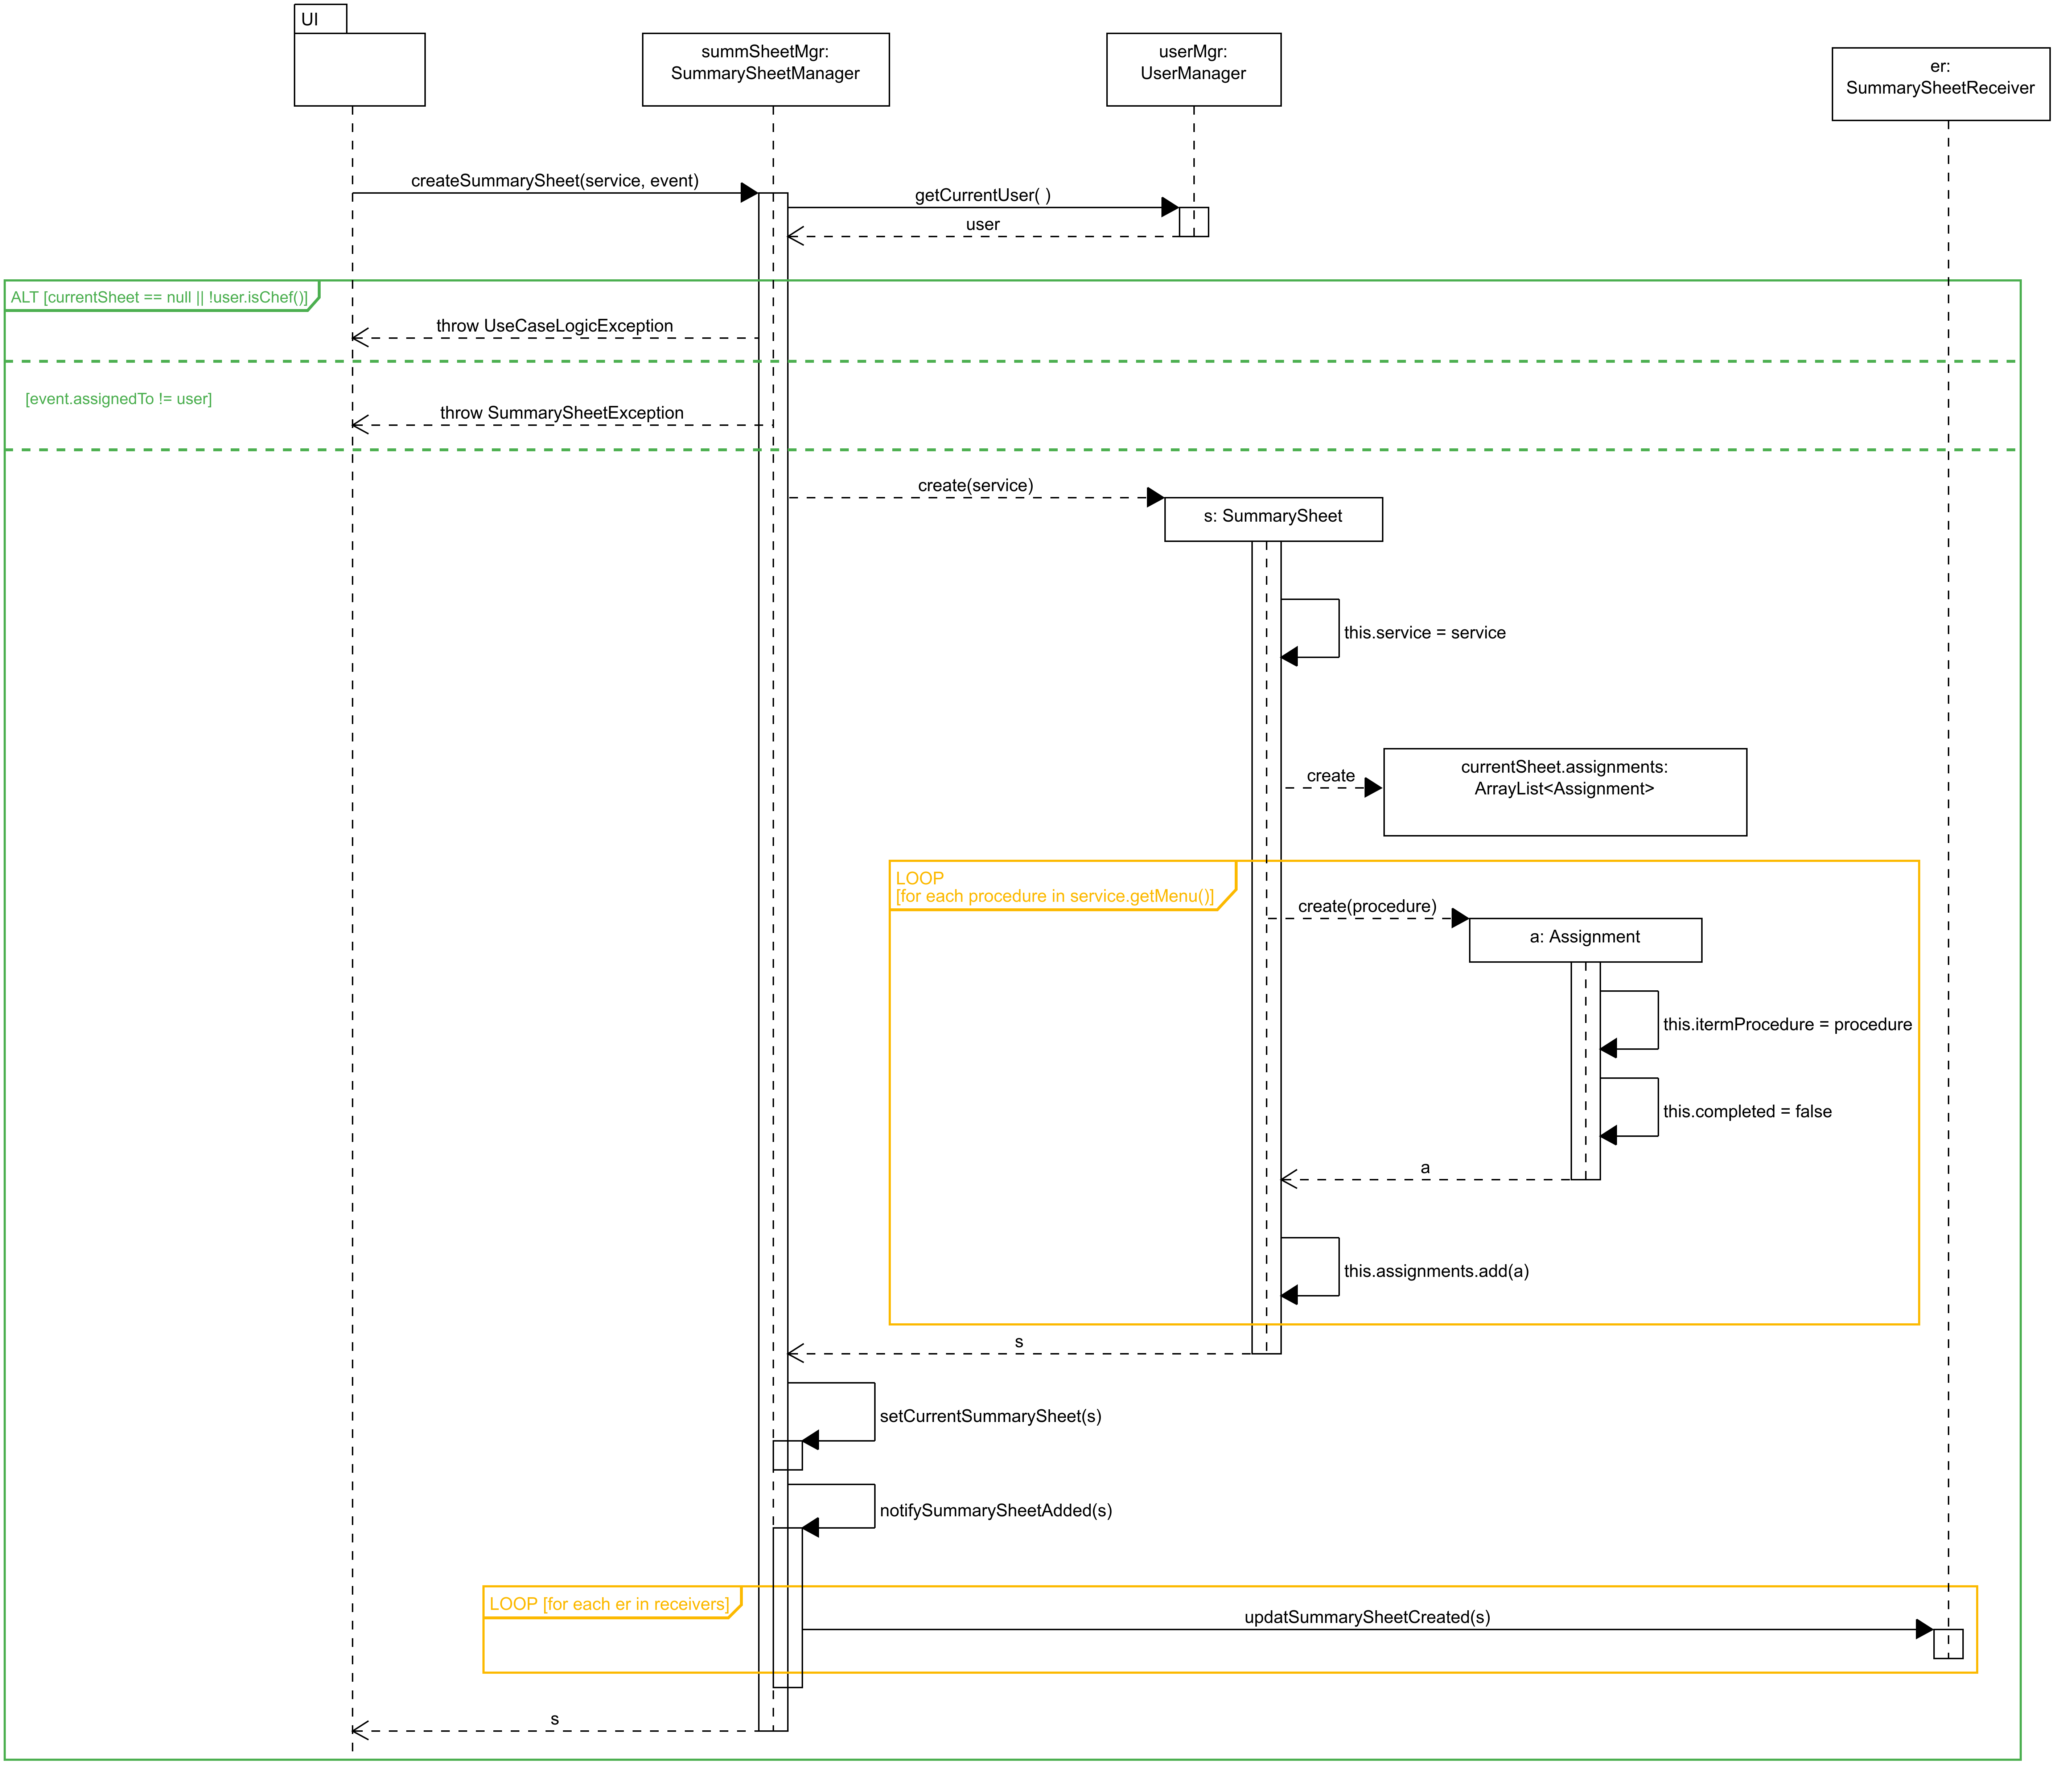
\includegraphics[max width=\textwidth, max height=138mm]{../resources/img/GCC/DSD/op1.png}

\subsection{chooseSummarySheet}
\centering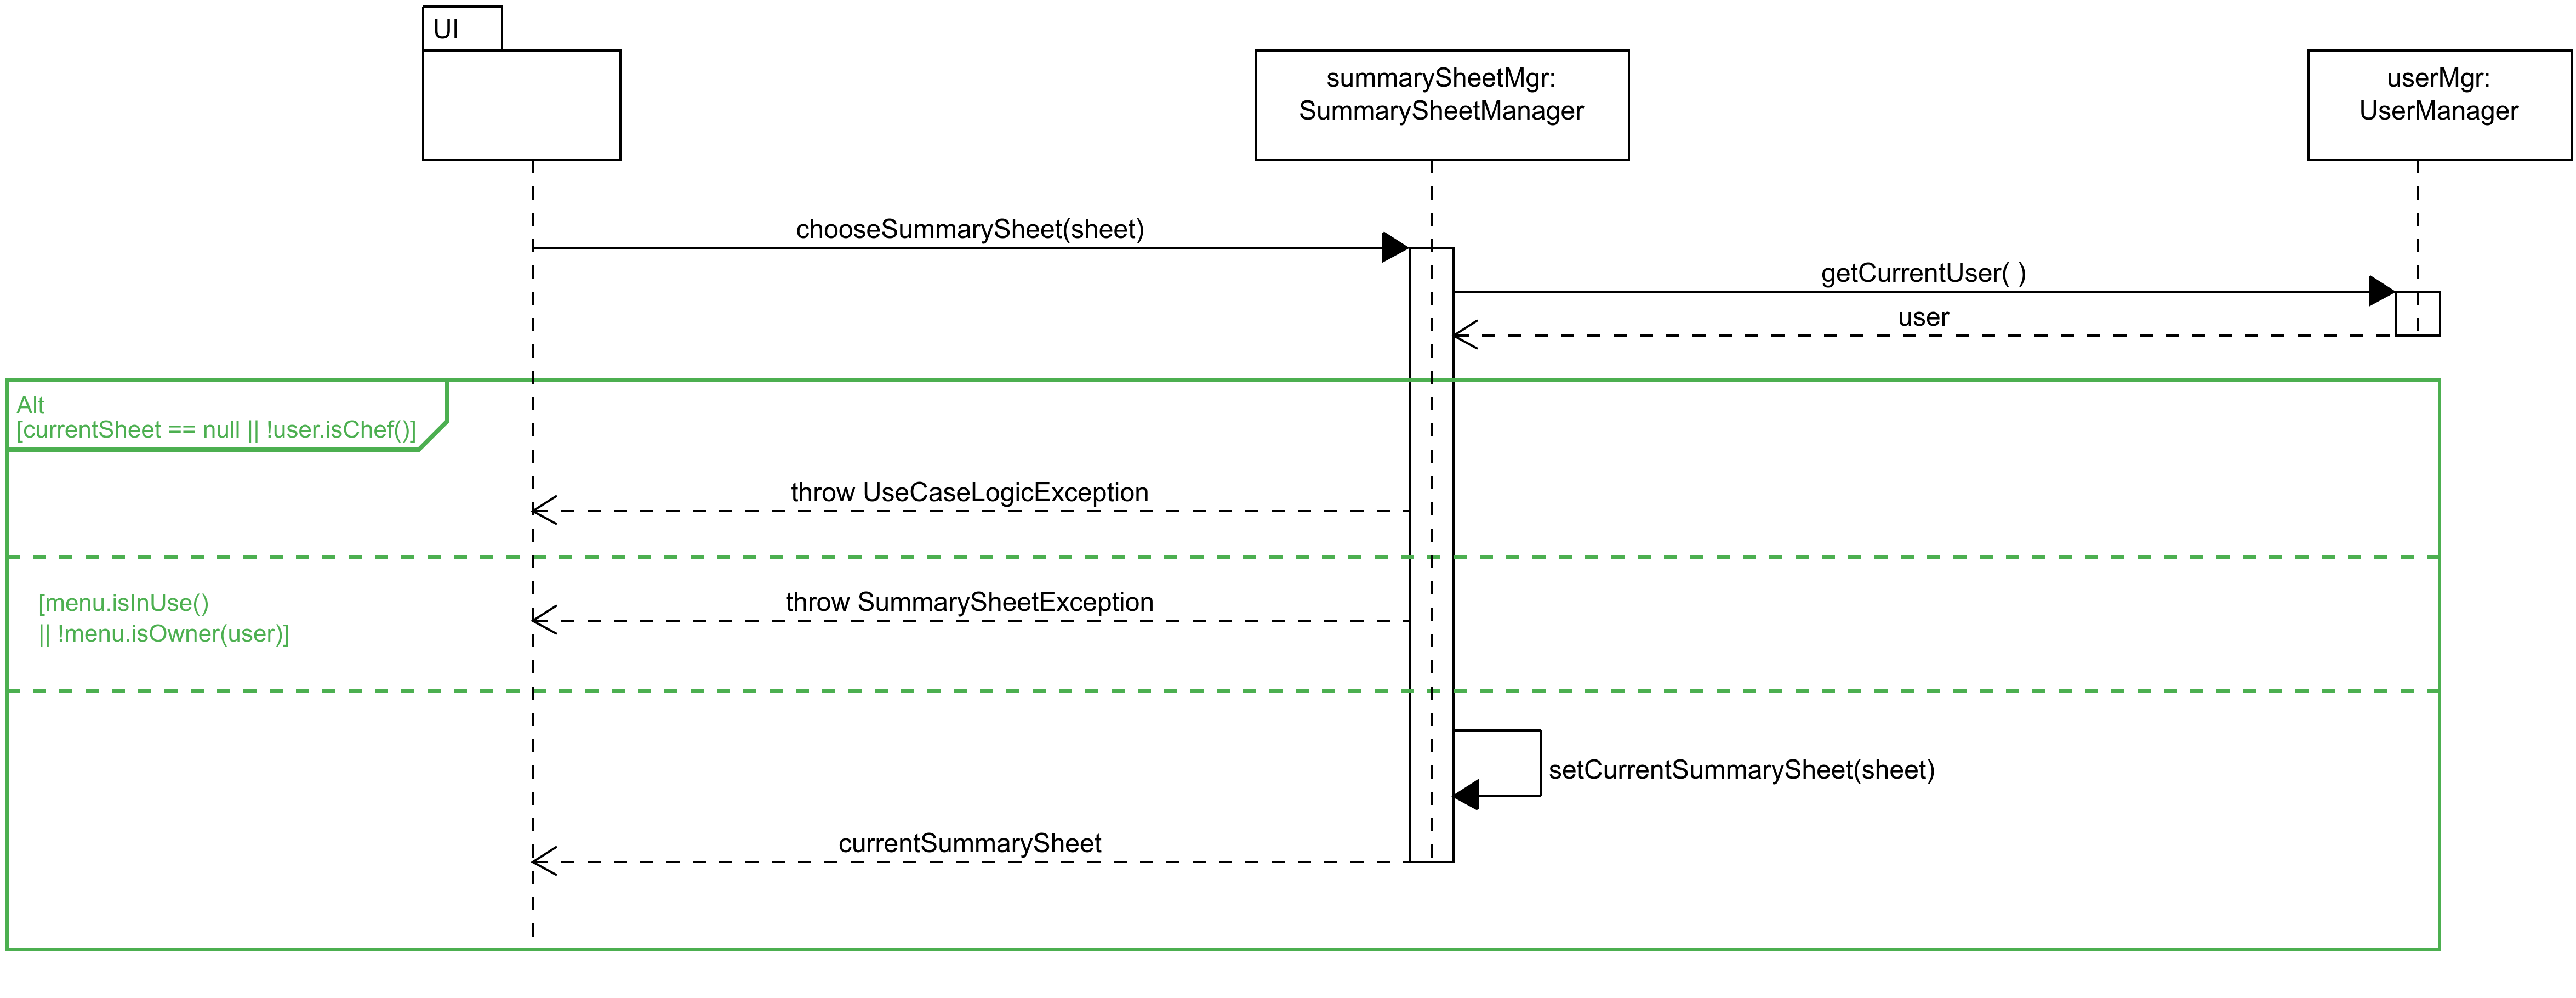
\includegraphics[max width=\textwidth, max height=190mm]{../resources/img/GCC/DSD/op1a.png}

\section{addProcedure}
\centering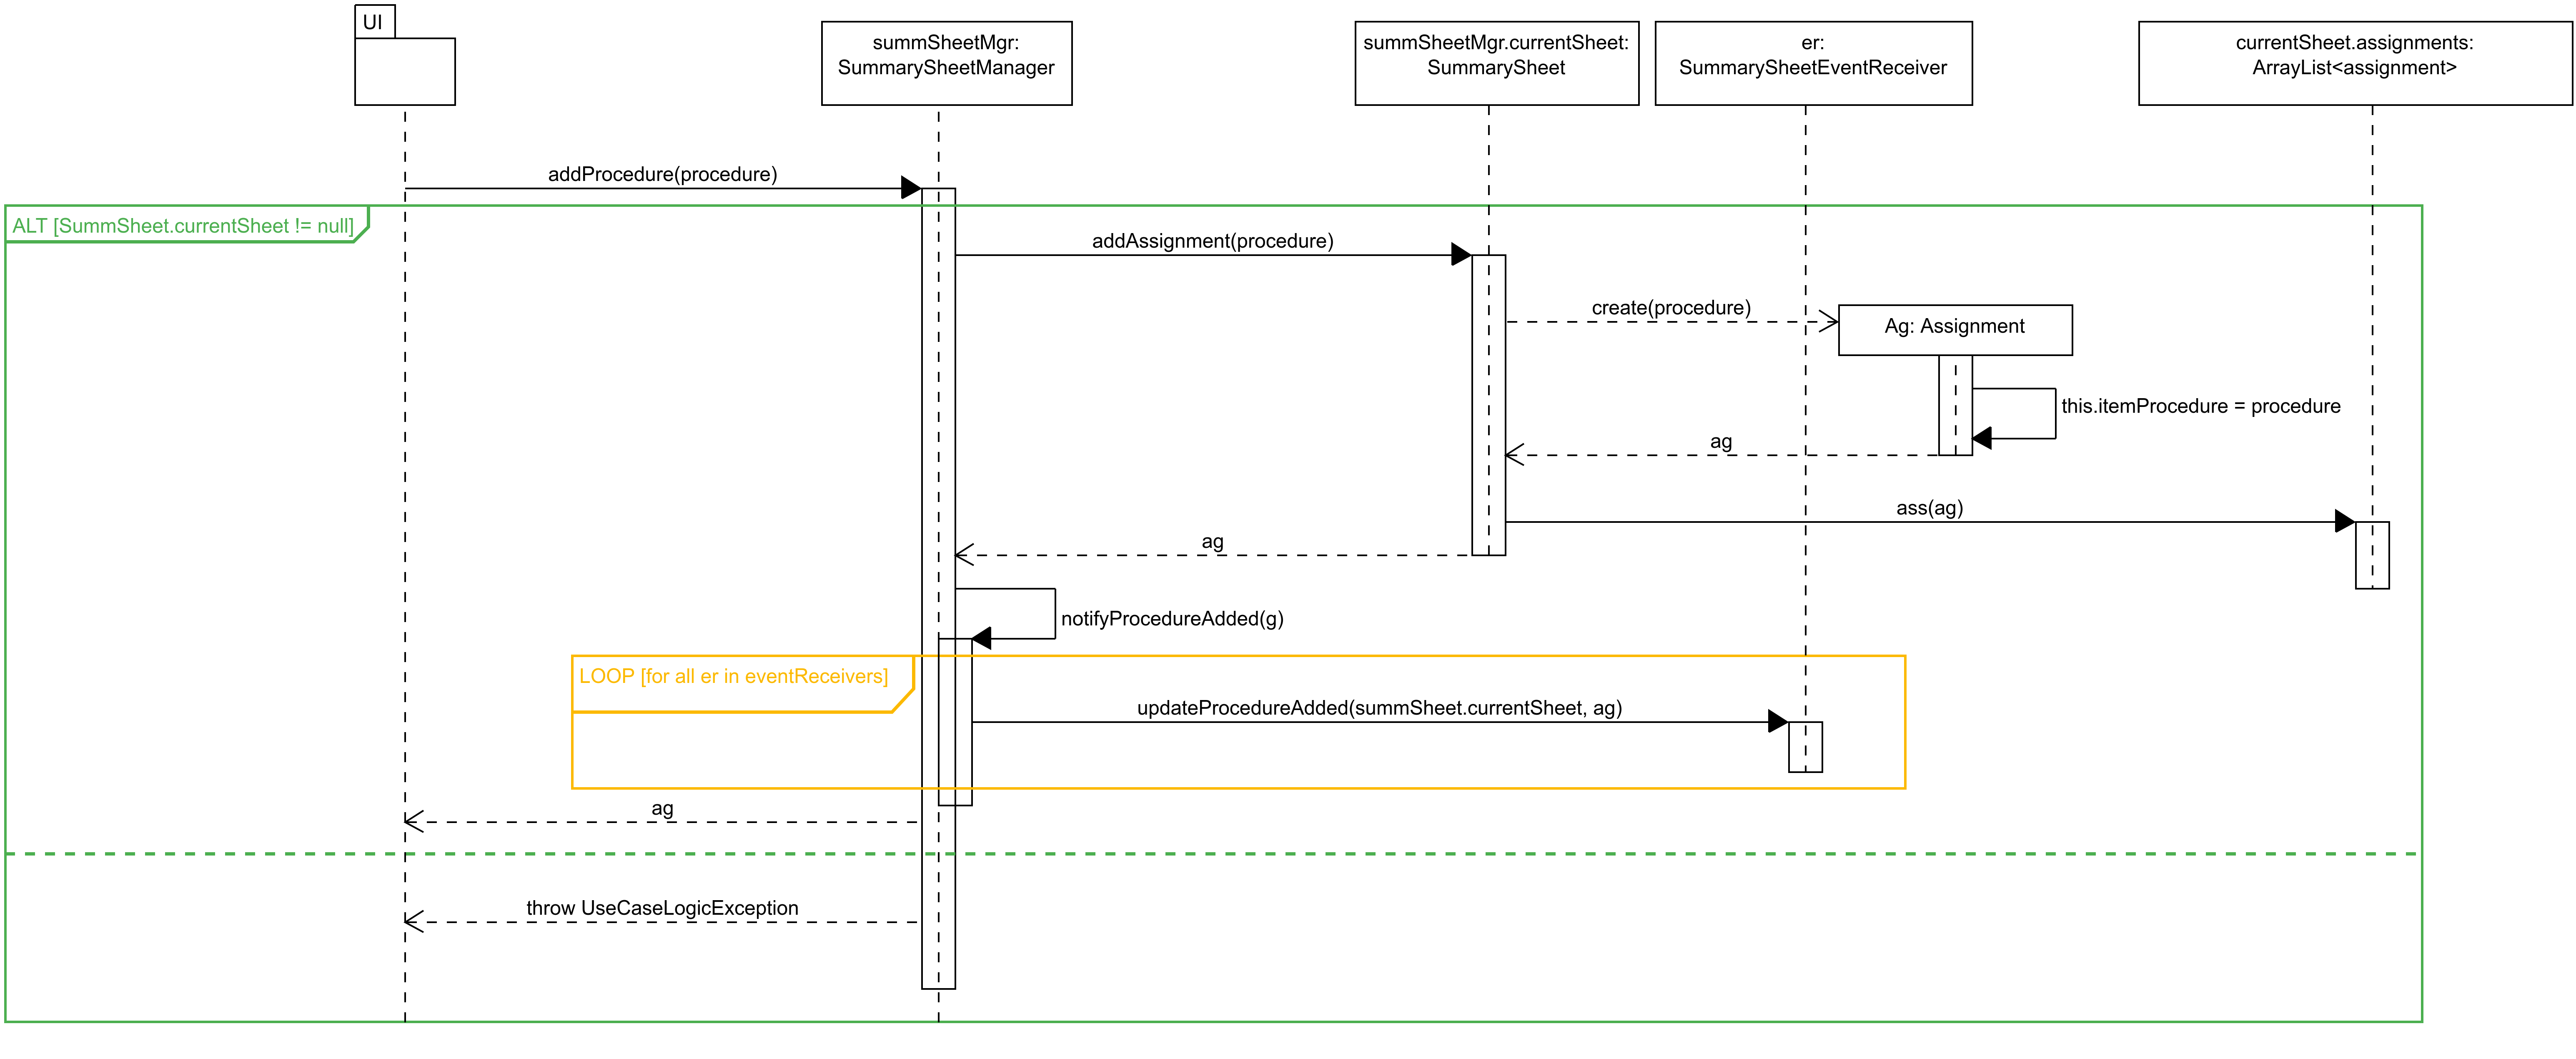
\includegraphics[max width=\textwidth, max height=190mm]{../resources/img/GCC/DSD/op2.png}

\subsection{removeProcedure}
\centering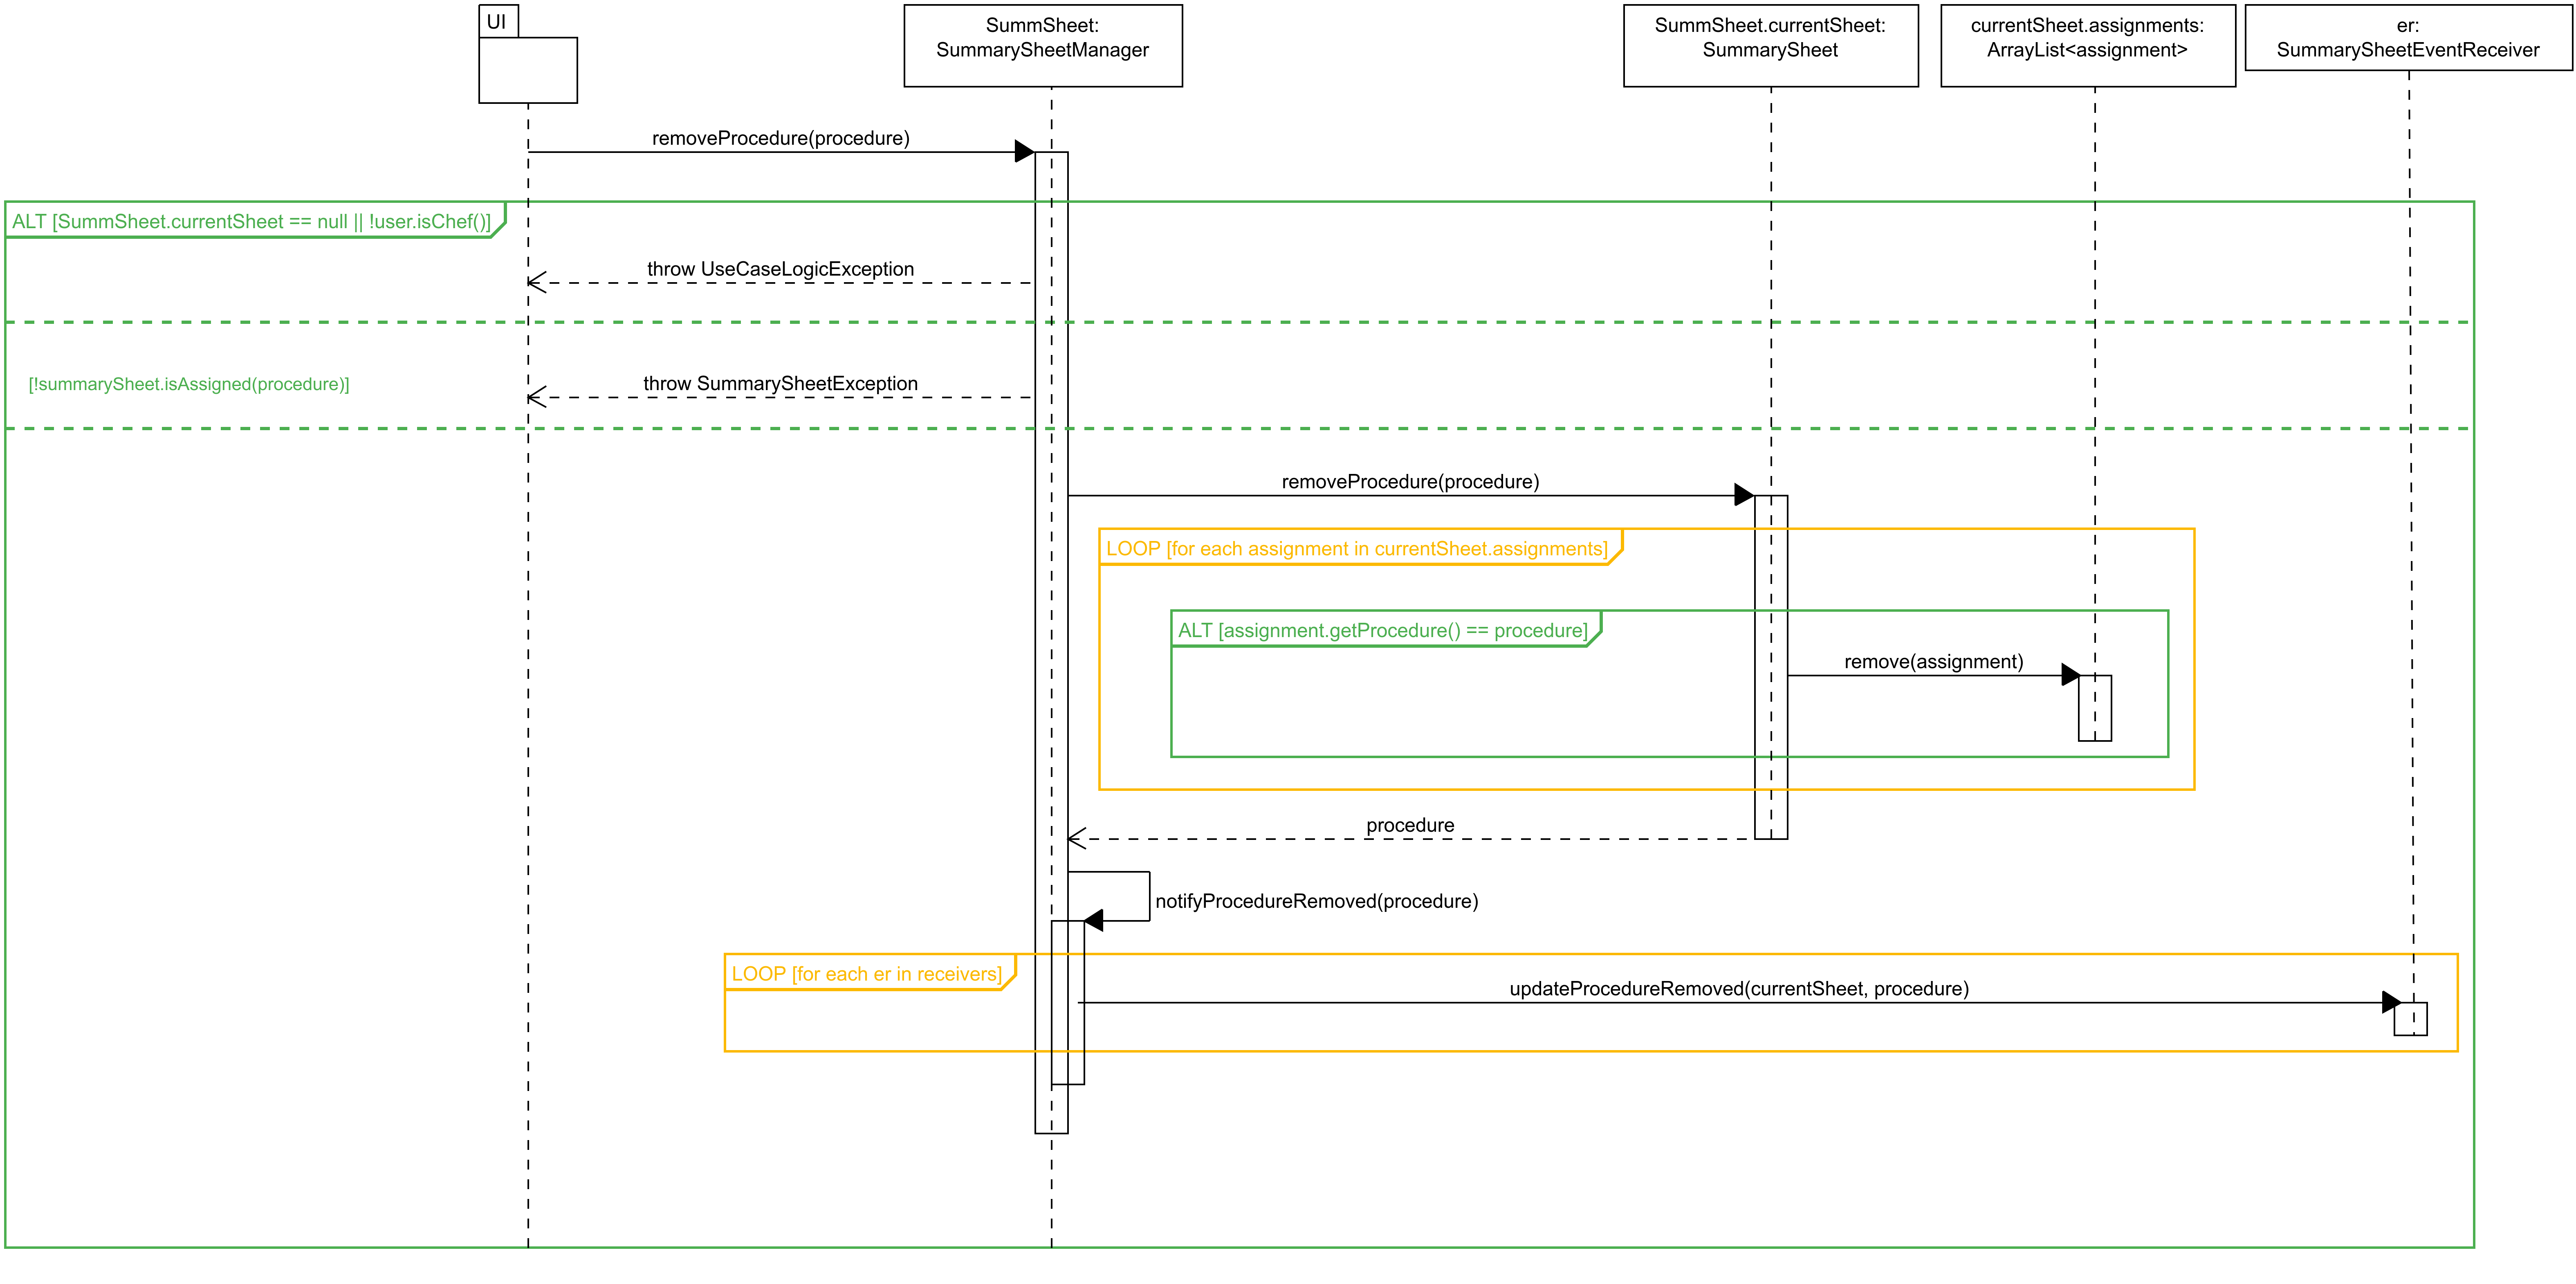
\includegraphics[max width=\textwidth, max height=190mm]{../resources/img/GCC/DSD/op2a.png}

\section{changeAssignmentOrder}
\centering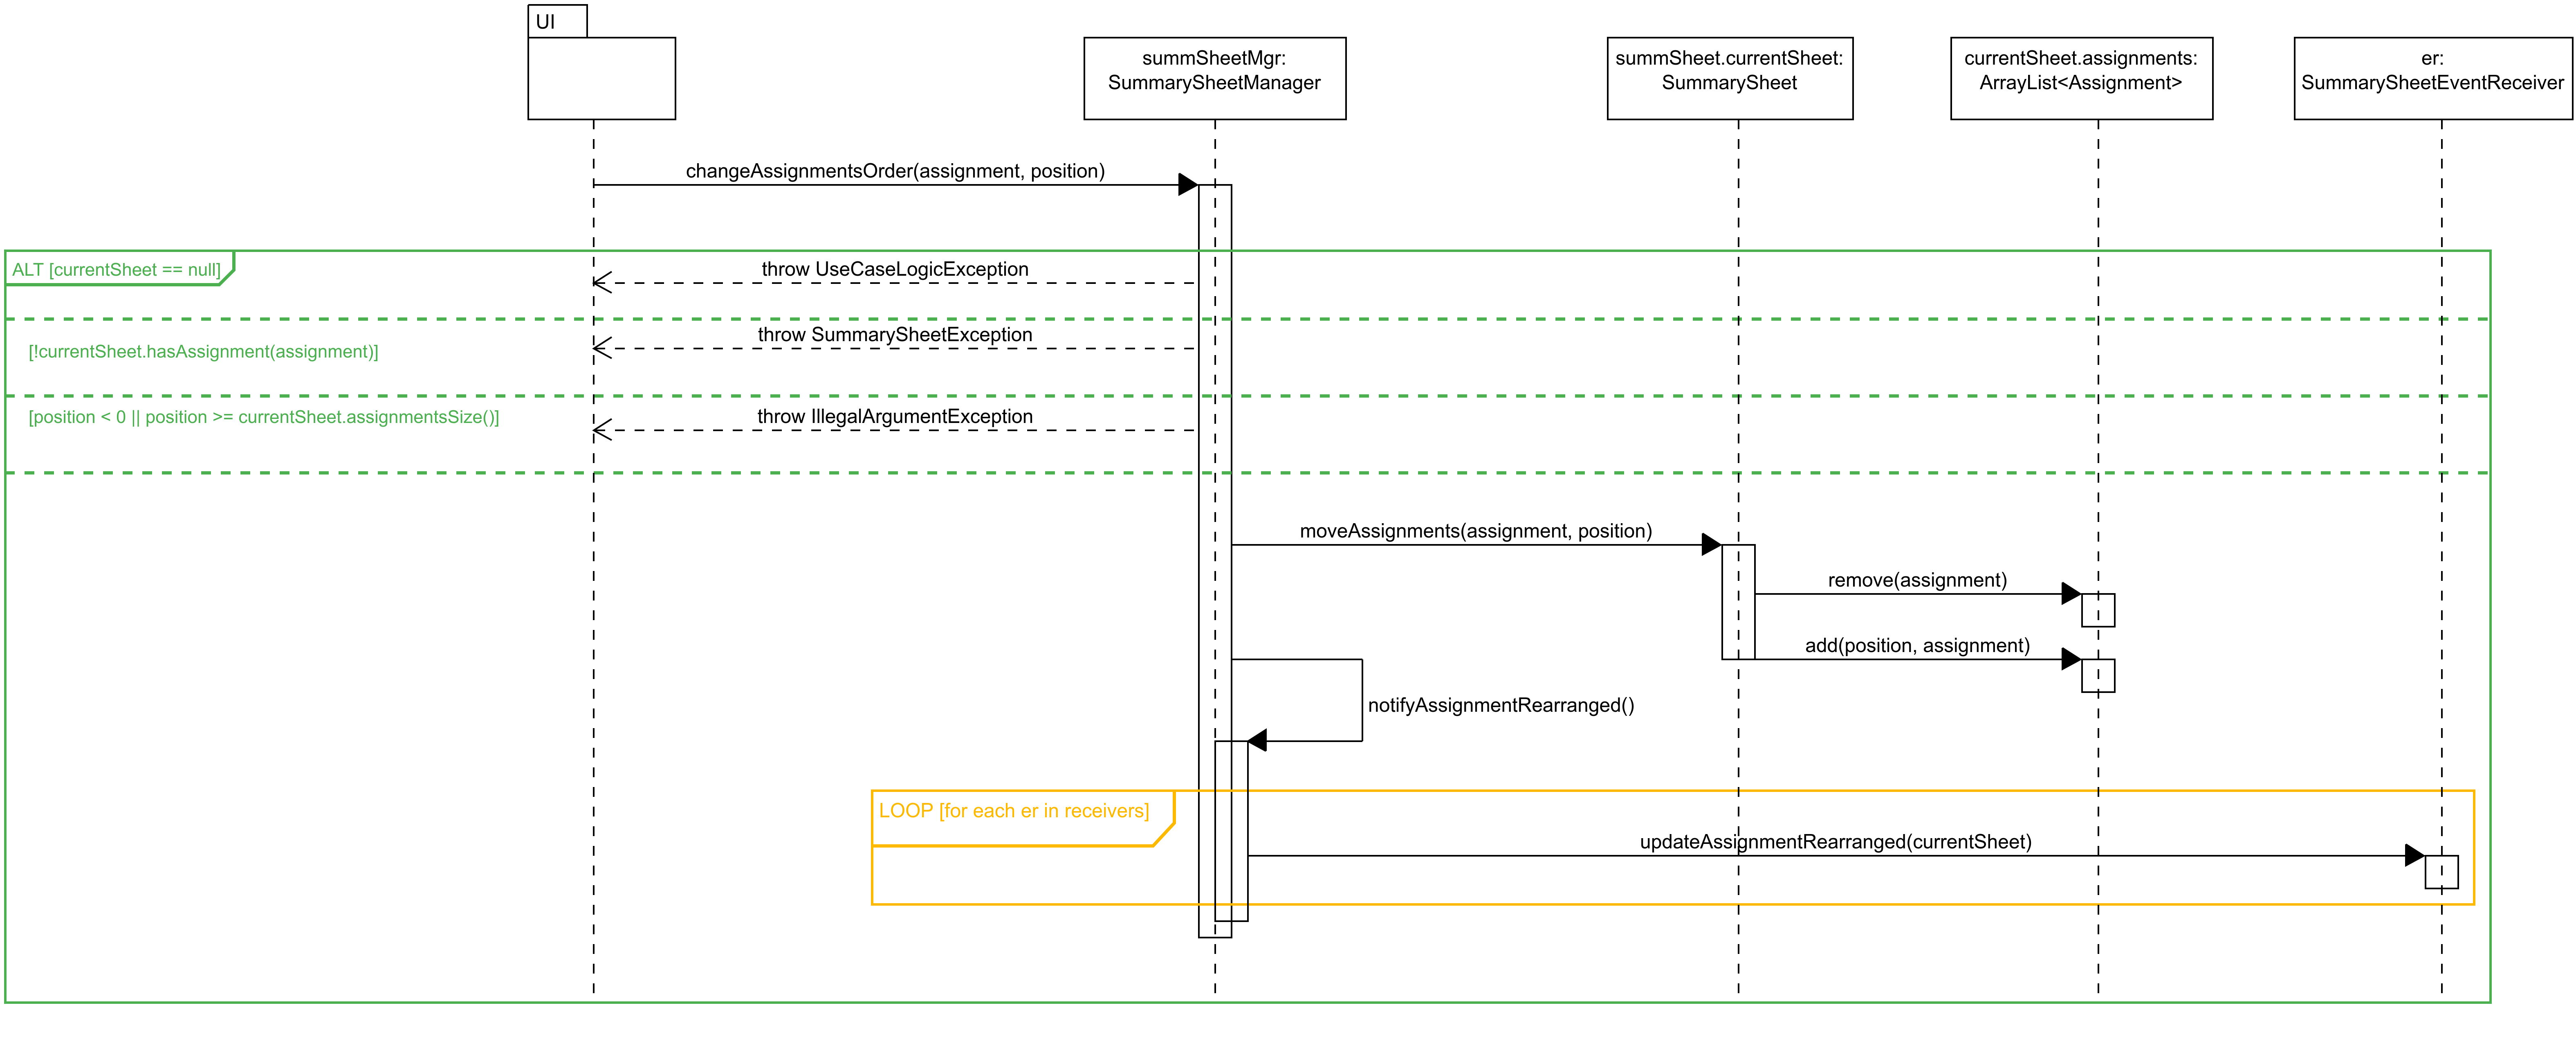
\includegraphics[max width=\textwidth, max height=190mm]{../resources/img/GCC/DSD/op3.png}

\section{getShiftBoard}
\centering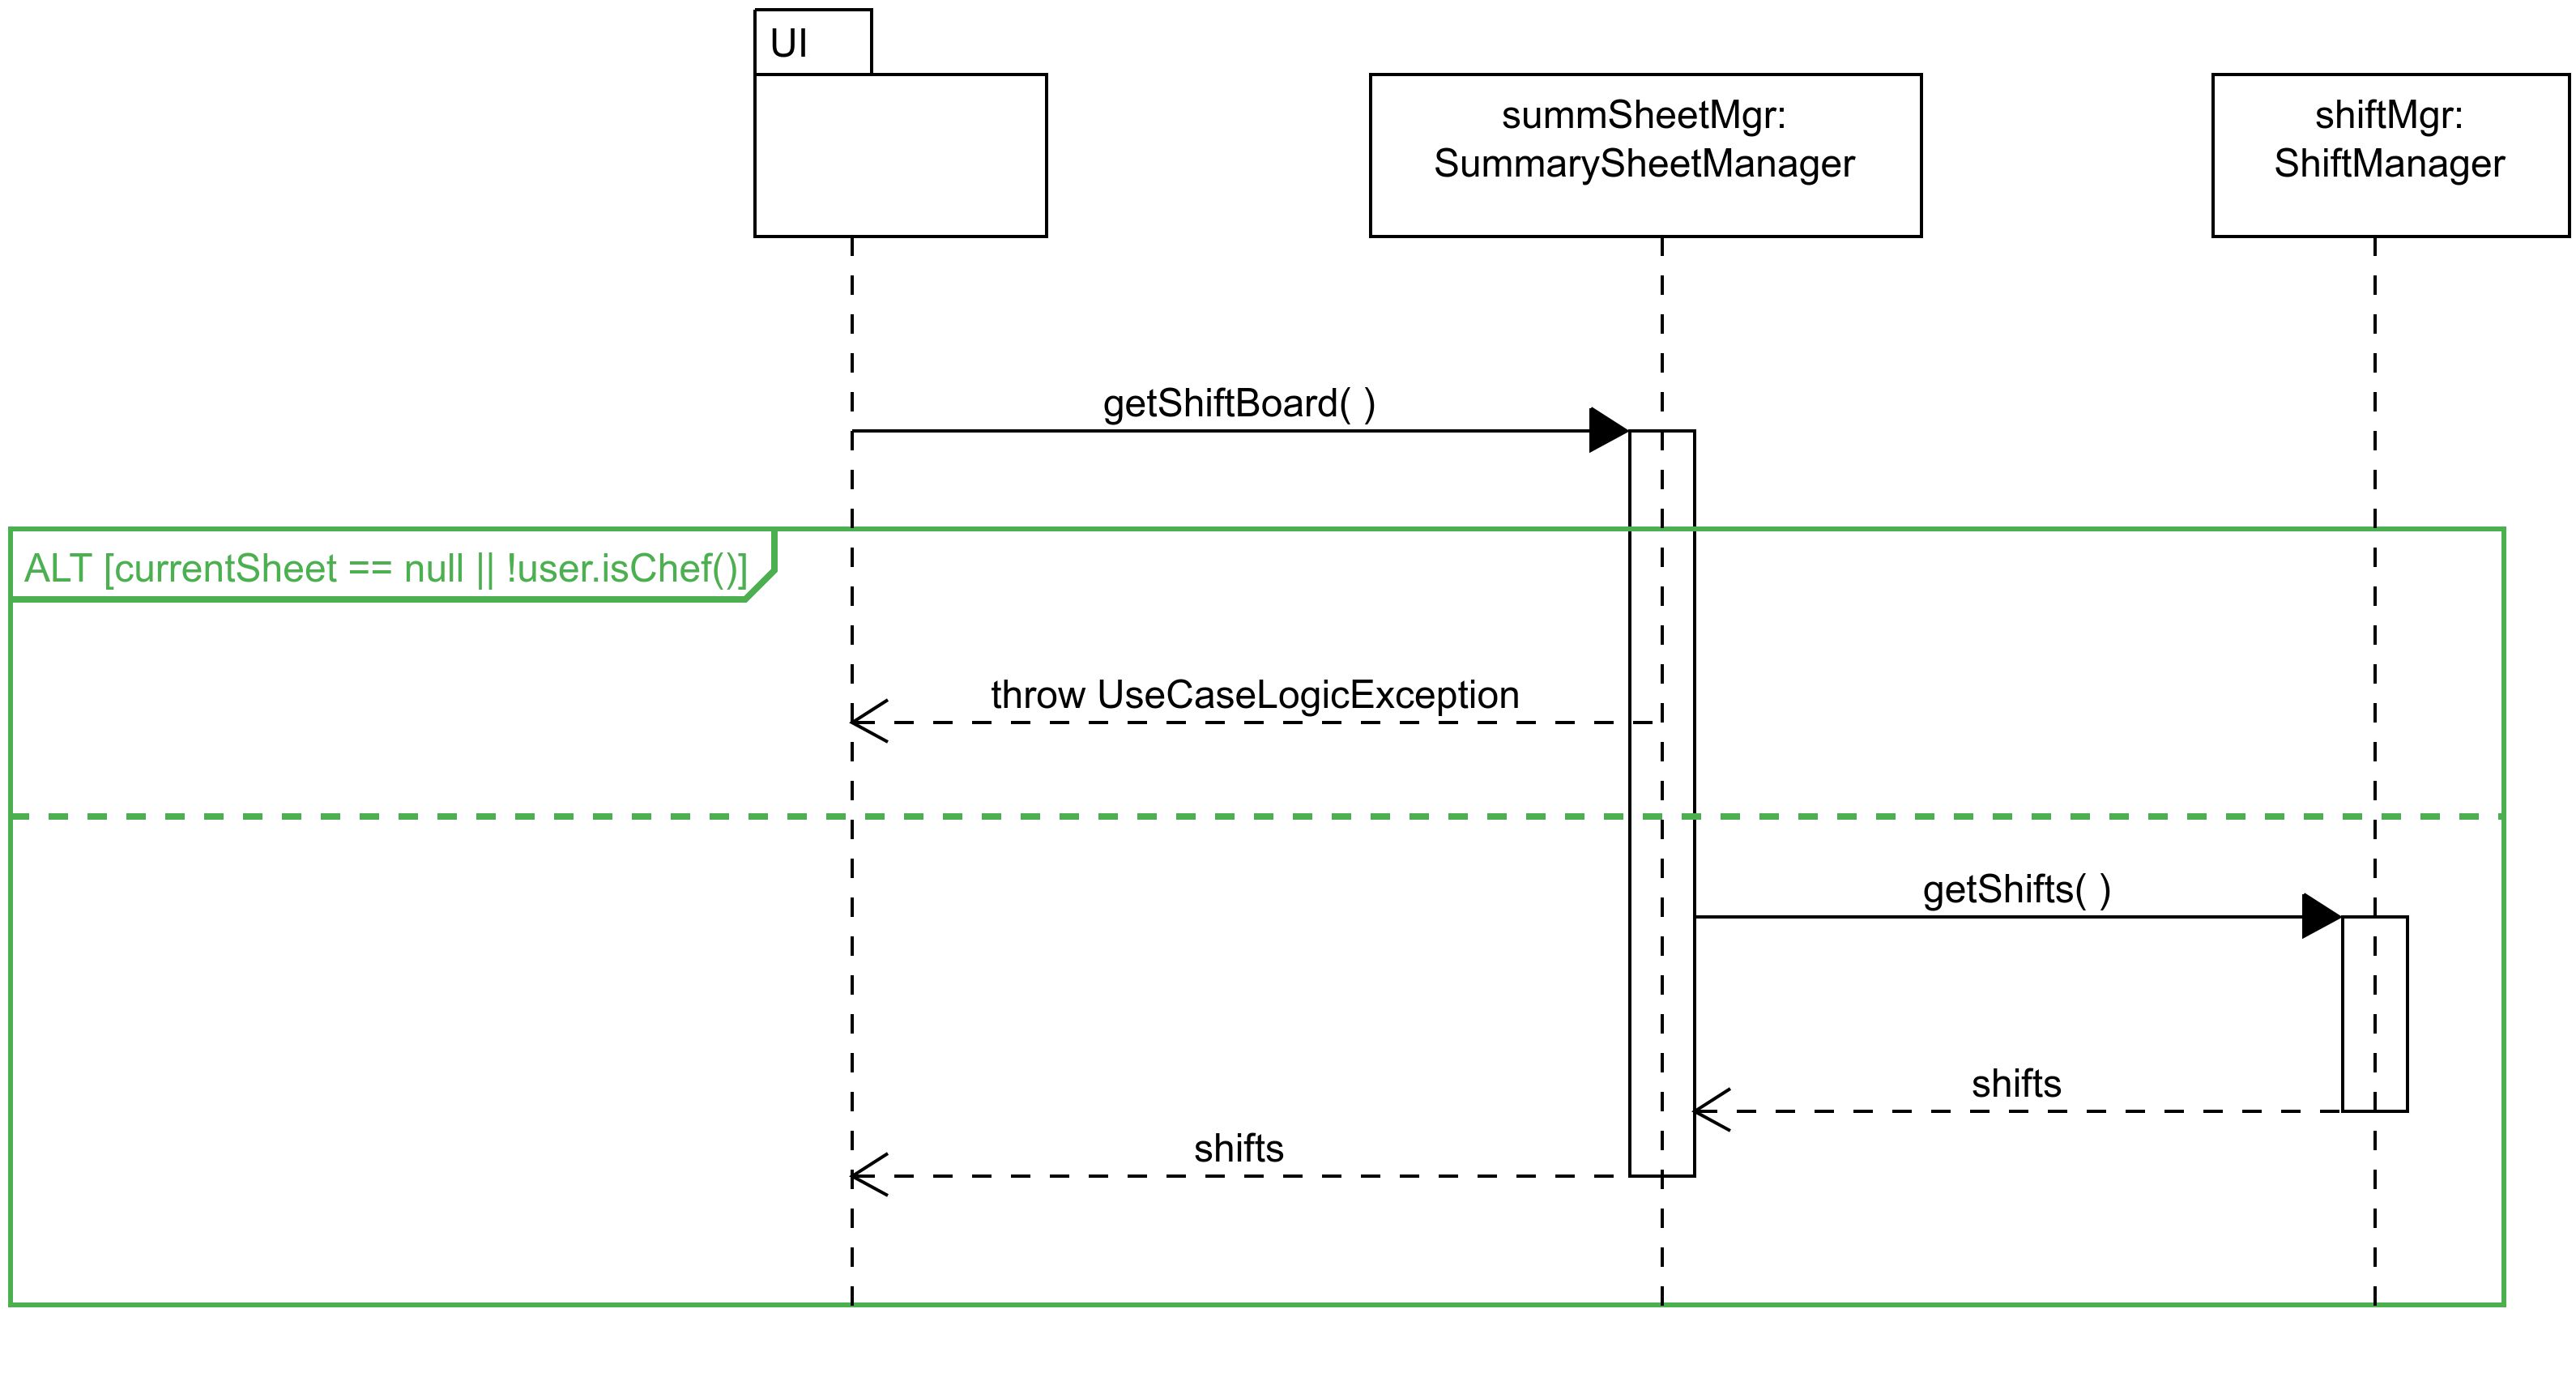
\includegraphics[max width=\textwidth, max height=190mm]{../resources/img/GCC/DSD/op4.png}

\section{defineAssignment}
\centering\includegraphics[max width=\textwidth, max height=190mm]{../resources/img/GCC/DSD/op5.png}

\subsection{procedureReady}
\centering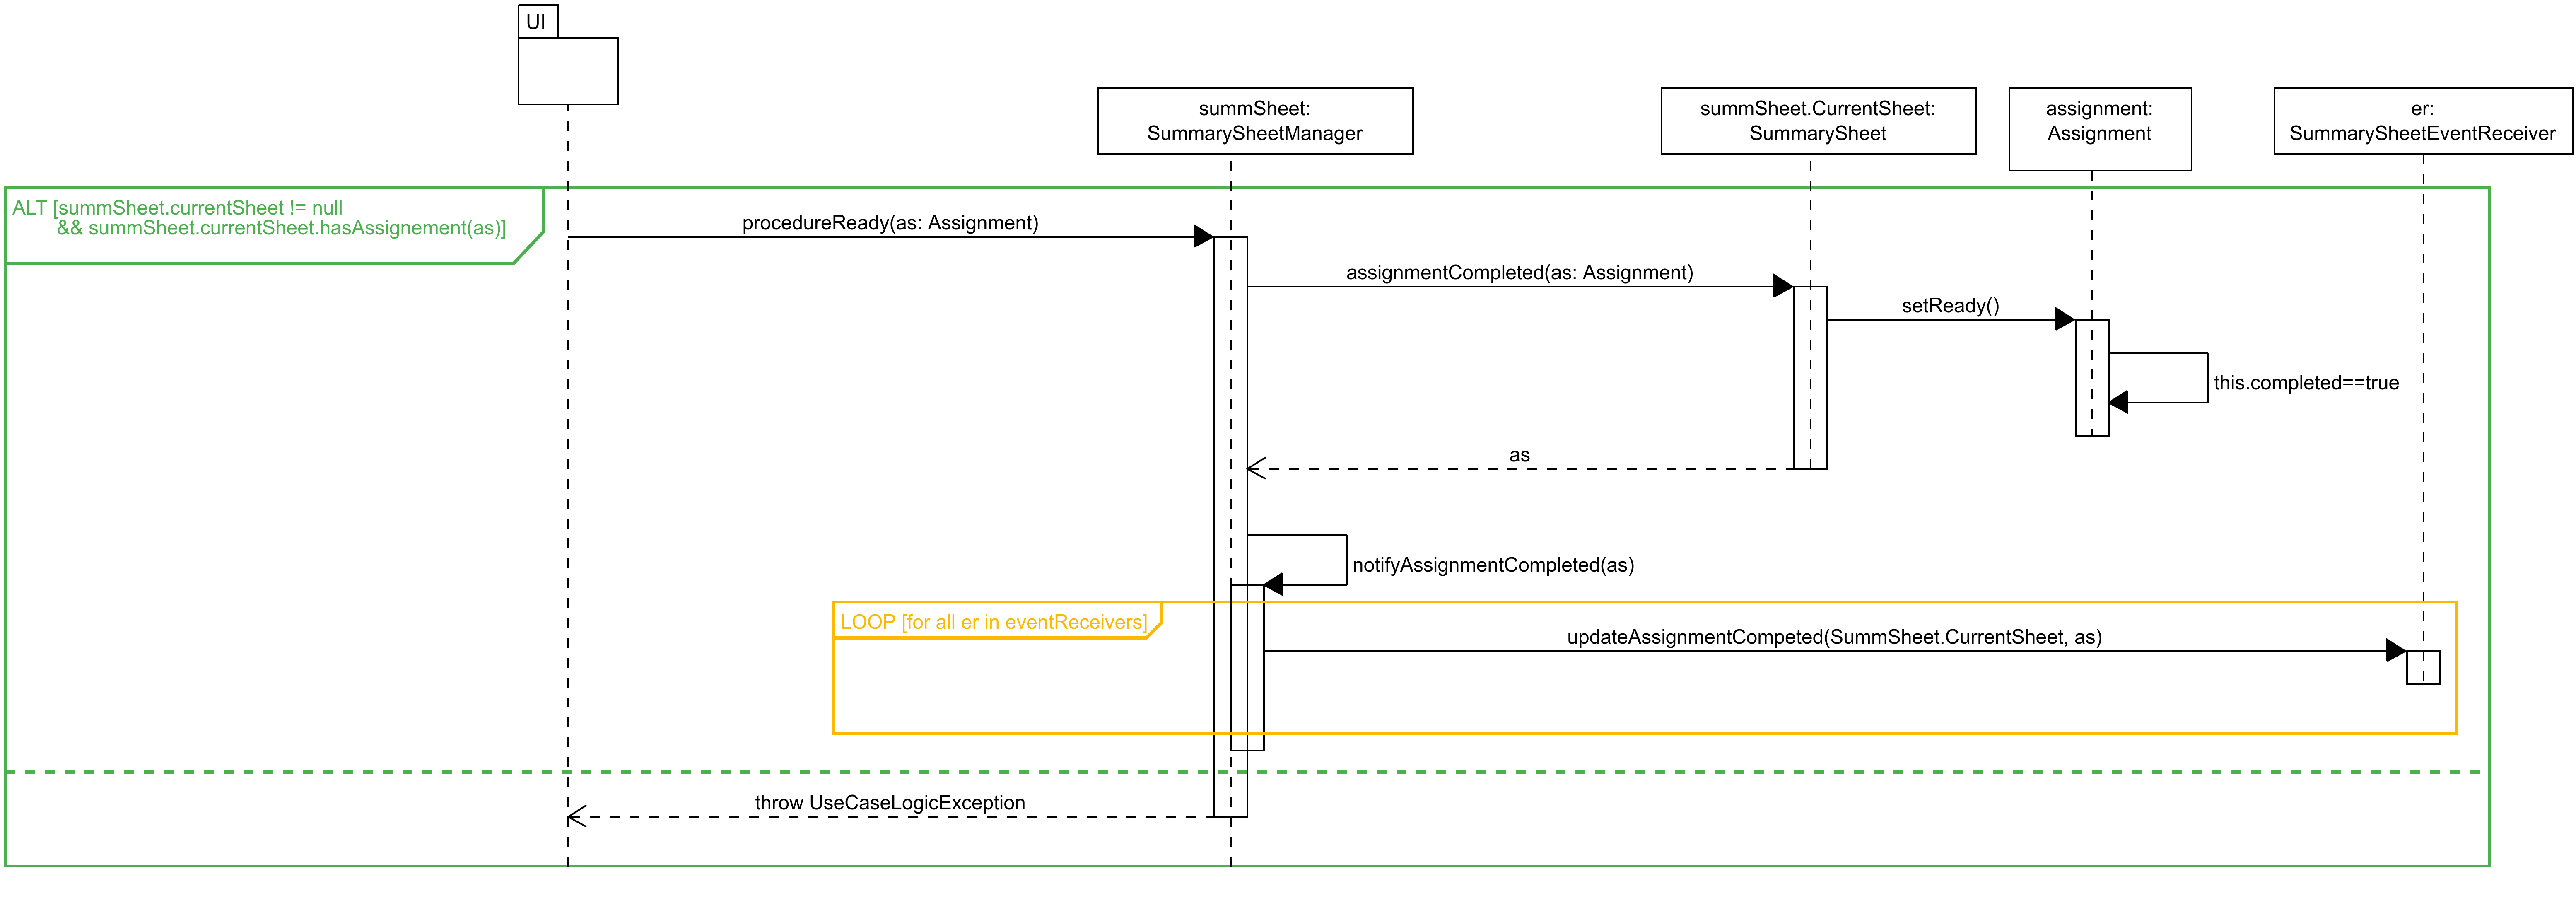
\includegraphics[max width=\textwidth, max height=190mm]{../resources/img/GCC/DSD/op5a.png}

\subsection{deleteAssignment}
\begin{figure}[H]
    \centering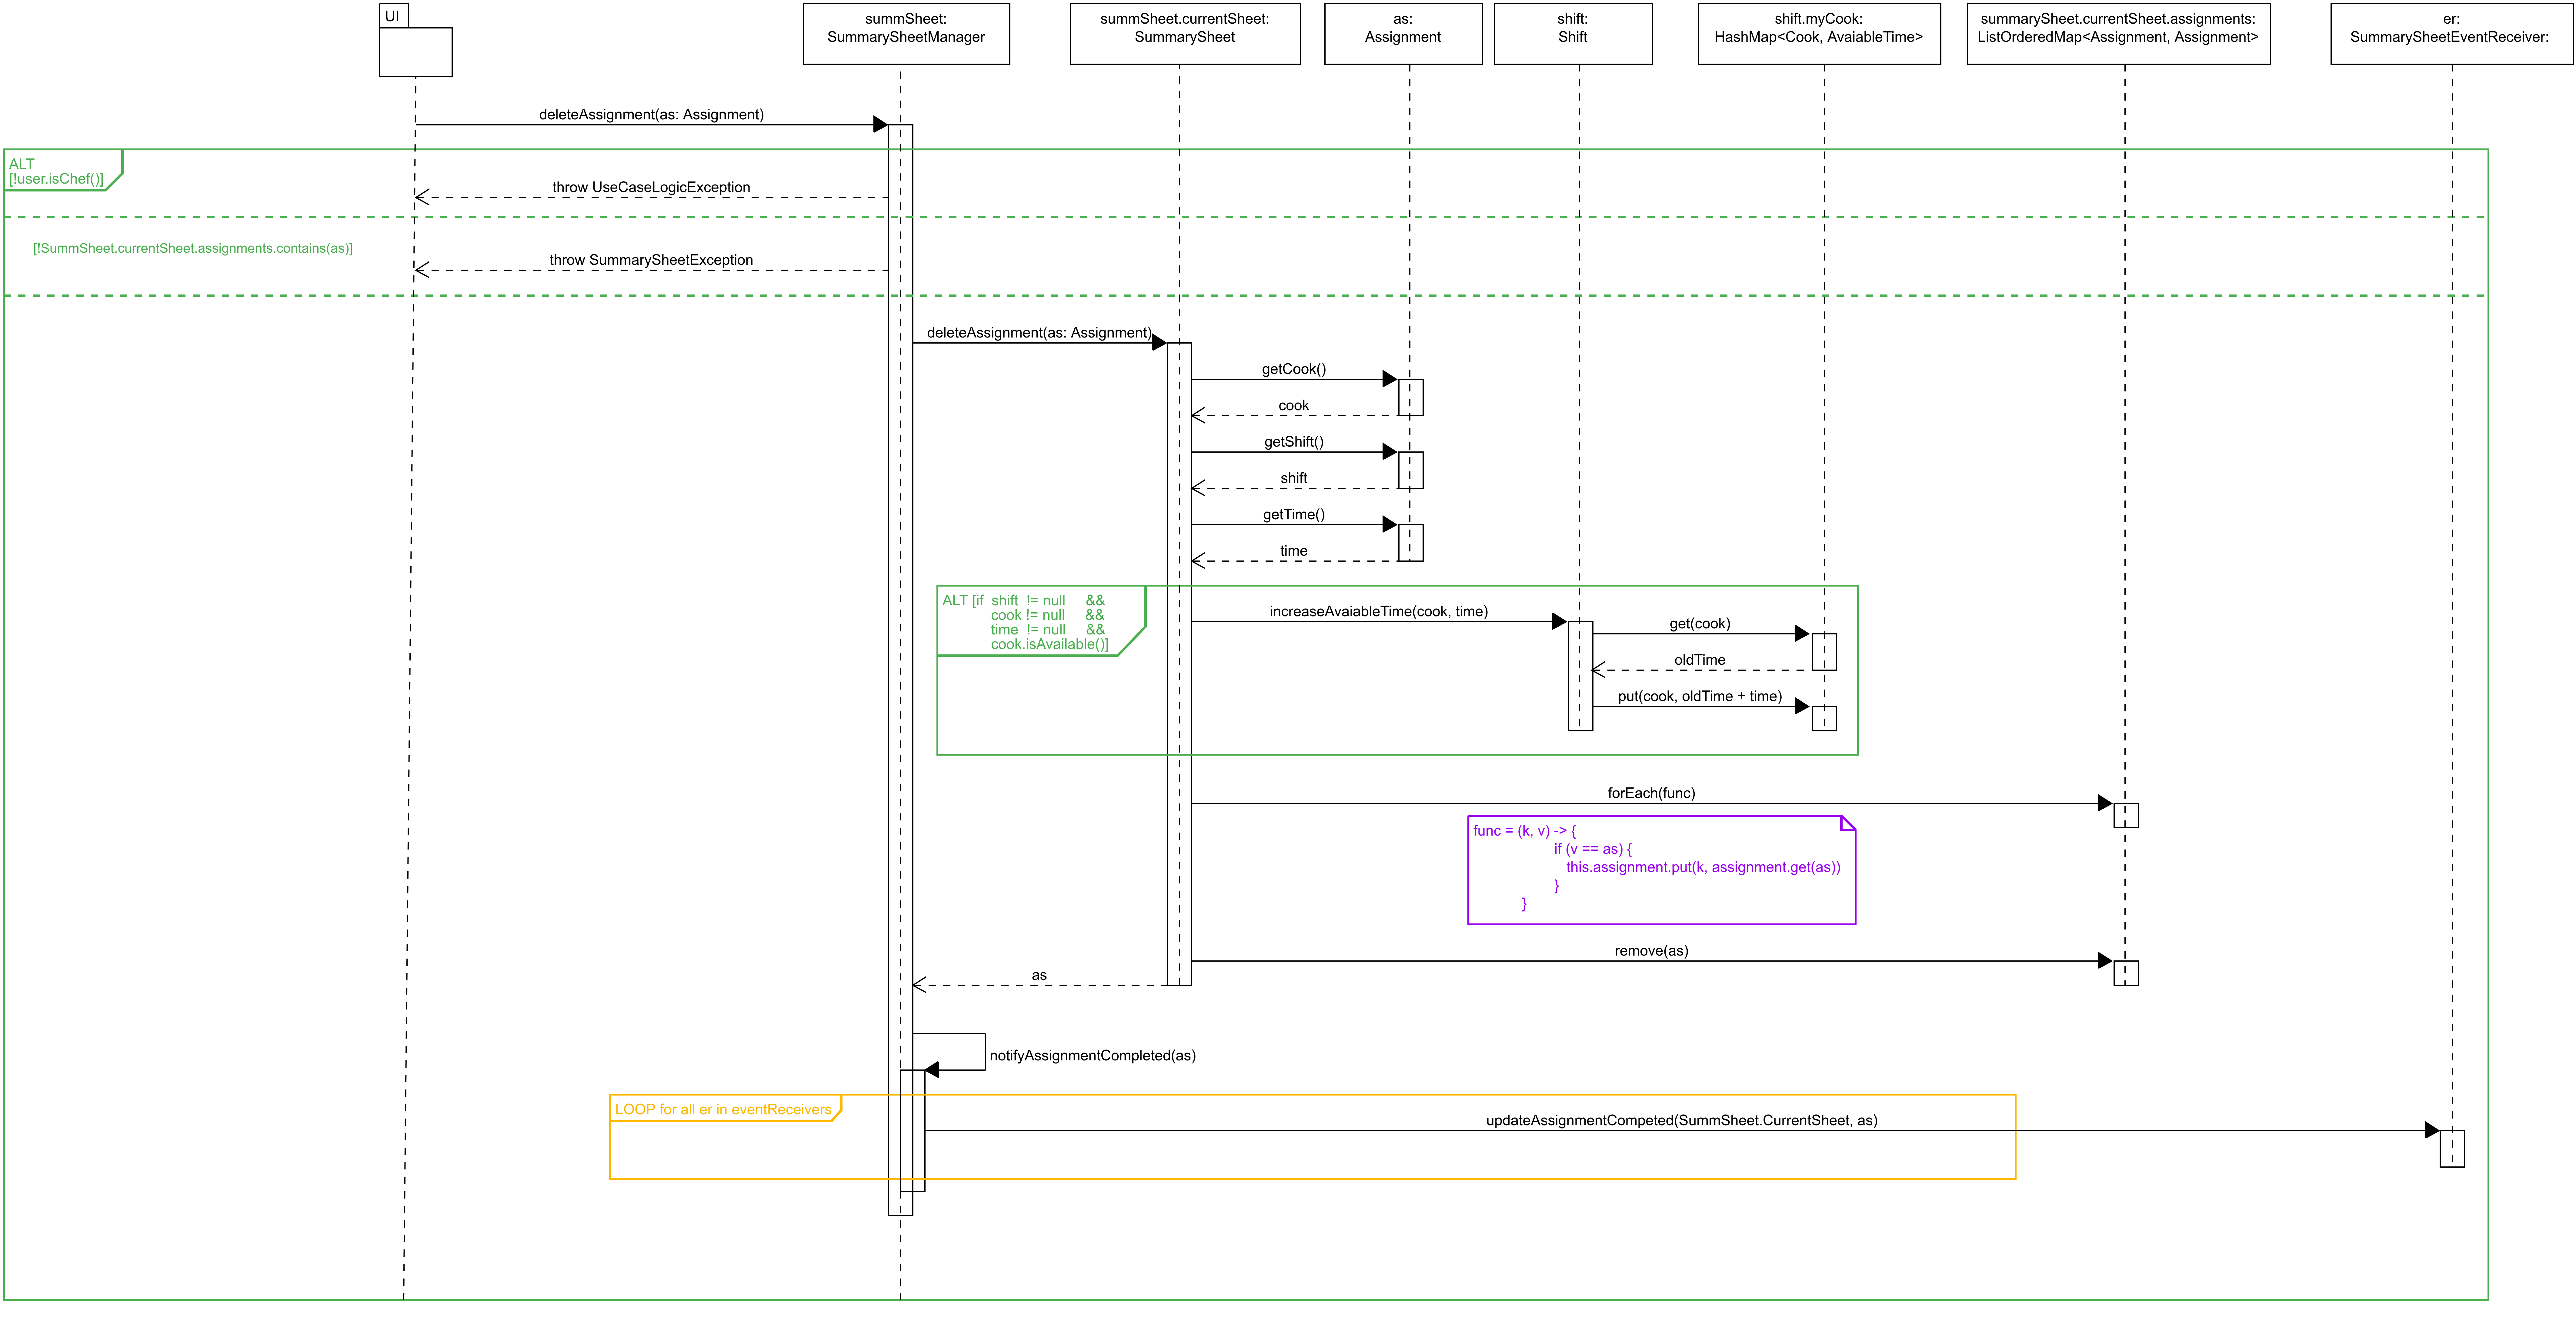
\includegraphics[max width=\textwidth, max height=190mm]{../resources/img/GCC/DSD/op5b.png}
\end{figure}

\normalpapersize
\chapter{Implementazione}
\end{document}